% Full manuscript assembly for TPS-ZKPI, typeset for the MDPI journal Blockchains.
% Build from this directory:
%   cd paper_mdpi && tectonic main.tex
% tectonic resolves the bibliography and reruns to convergence in a single pass.
%
% The IEEEtran/BRAINS 2026 version of this manuscript lives in ../paper and is
% maintained independently; body text is duplicated, not shared.
%
% Front matter, intro, related work, problem/threat model, design, discussion, and
% conclusion are modular .tex files. The Evaluation chapter is the authoritative modular
% evaluation (evaluation.tex) with numbers transcribed from the deterministic
% multi-seed result files; see ../paper/README.md for provenance.
%=================================================================
\documentclass[blockchains,article,submit,moreauthors]{Definitions/mdpi}

%=================================================================
% MDPI internal commands - do not modify
\firstpage{1}
\makeatletter
\setcounter{page}{\@firstpage}
\makeatother
\pubvolume{1}
\issuenum{1}
\articlenumber{0}
\pubyear{2026}
\copyrightyear{2026}
\datereceived{ }
\dateaccepted{ }
\datepublished{ }

%=================================================================
% mdpi.cls already loads: amsmath, amssymb, amsthm, booktabs, tabularx, multirow,
% graphicx, float, natbib, hyperref, cleveref, caption, subfig. Only additions go here.

% --- graphics ---
\graphicspath{{figures/}{./}}

% The MDPI class hardcodes .eps for its logos, which the XeTeX-based tectonic engine
% cannot read. Definitions/logo-{mdpi,updates}.eps hold PDF bytes under the .eps name;
% this rule tells graphicx to parse them with the PDF reader.
\DeclareGraphicsRule{.eps}{pdf}{*}{}

% --- misc ---
\usepackage{pifont}
\usepackage{longtable}
\usepackage{placeins} % \FloatBarrier, used before the references
\newcommand{\cmark}{\ding{51}}
\newcommand{\xmark}{\ding{55}}

% Table notes: legends, abbreviations, and dagger notes set below a table. Undo the
% float's \centering so that multi-line notes are justified rather than centered.
\newenvironment{tablenote}{\par\vspace{0.4em}\footnotesize
  \leftskip=0pt\rightskip=0pt\parfillskip=0pt plus 1fil\parindent=0pt}{\par}

% Keep consecutive tables together near the top of float-only pages instead of
% stretching the inter-float glue across the full page.
\makeatletter
\setlength{\@fptop}{0pt}
\setlength{\@fpsep}{12pt plus 2pt}
\setlength{\@fpbot}{0pt plus 1fil}
\makeatother
\setcounter{topnumber}{5}
\setcounter{totalnumber}{6}
\renewcommand{\topfraction}{0.95}
\renewcommand{\textfraction}{0.05}
\renewcommand{\floatpagefraction}{0.80}

% Long identifiers such as controlled\_difference are single unbreakable words, and the
% single-column MDPI text block is narrower than IEEEtran's two-column measure. Permit a
% break after the underscore so they wrap instead of running into the margin. No hyphen
% is inserted: it would be indistinguishable from part of the identifier. This affects
% only the \_ text command, not math subscripts.
\DeclareRobustCommand{\_}{\textunderscore\discretionary{}{}{}}

% A paragraph with no acceptable line break, such as one that opens with a long
% hyphenated name, would otherwise run into the margin. Emergency stretch is used
% only for those paragraphs; all others are typeset as before.
\setlength{\emergencystretch}{1.5em}

% --- shorthand macros (from the source manuscript) ---
\newcommand{\negl}{\mathsf{negl}}
\newcommand{\Com}{\mathsf{Com}}
\newcommand{\Eval}{\mathsf{Eval}}
\newcommand{\Verify}{\mathsf{Verify}}
\newcommand{\Enc}{\mathsf{Enc}}
\newcommand{\Setup}{\mathsf{Setup}}
\newcommand{\Prove}{\mathsf{Prove}}
\newcommand{\Pad}{\mathsf{Pad}}
\newcommand{\Quantile}{\mathsf{Quantile}}
\newcommand{\Acc}{\mathsf{Acc}}

%=================================================================
% Title, authors, abstract, keywords. MDPI declares these in the preamble.
% Title, authors, abstract, keywords. MDPI declares all of these in the PREAMBLE,
% so main.tex \inputs this file before \begin{document}.
\Title{Enhancing Consent Policy Privacy in Blockchain-Based Healthcare Data Sharing}

% TODO(author): confirm affiliation numbering and add ORCID iDs (\orcidA{} etc.).
% The trailing `,`* marks the corresponding author.
\Author{Kun Li $^{1,}$*, Ankur Lohachab $^{1}$, Michel Dumontier $^{1}$ and Visara Urovi $^{1}$}

% MDPI internal command: authors for the PDF metadata.
\AuthorNames{Kun Li, Ankur Lohachab, Michel Dumontier and Visara Urovi}

\address{%
	$^{1}$ \quad Department of Advanced Computing Sciences, Maastricht University, 6200 MD Maastricht, The Netherlands; ankur.lohachab@maastrichtuniversity.nl (A.L.); michel.dumontier@maastrichtuniversity.nl (M.D.); v.urovi@maastrichtuniversity.nl (V.U.)}

\corres{Correspondence: k.li@maastrichtuniversity.nl}

% MDPI requires a single paragraph, so this abstract carries no blank lines.
% Condensed (~200 words) from the IEEEtran version in ../paper/sec_frontmatter.tex.
\abstract{
	Public-chain consent enforcement in healthcare data sharing can expose governing policies through transaction artifacts even when health data are encrypted.
	Hiding policy logic alone leaves policy-dependent metadata observable.
	To address this gap, we present the Trusted Proof Service-assisted Zero-Knowledge Policy Interpreter (TPS-ZKPI), which delegates private proof generation to a trusted service while verifying compliance with committed, bounded Boolean consent policies on-chain.
	Fixed-length encoding, commitment binding, and a reusable interpreter make the proof interface policy-independent, while transcript normalization limits variation in calldata, event shape, and gas for the evaluated policies.
	We assess the resulting public transcript on Polygon Amoy using generated policies and supervised and unsupervised attacks that model a passive public-chain metadata observer. Of $45$ supervised tasks, $43$ stay below our multi-seed leakage criterion. Diagnostics link the two threshold crossings to chance correlations between policy labels and independently drawn padding targets. A paired ablation further shows that padding suppresses policy-correlated gas signals on the evaluated subset, with mean gas overheads of about $46\%$ for access and $38\%$ for policy commitment.
	Together, these results support reduced leakage through the modeled metadata channels within the tested policy class and under the trusted-service assumption.
}

% MDPI keywords are semicolon-separated.
\keyword{blockchain; consent policy privacy; zero-knowledge proofs; Data Use Ontology (DUO); healthcare data sharing; metadata leakage}


%=================================================================
\begin{document}

\section{Introduction}
\label{sec:introduction}

Blockchain technology has emerged as a promising foundation for decentralized and auditable healthcare data sharing~\cite{kakarlapudi2021systematic, welzel2025enabling, li2024you}.
Its transparency and immutability allow consent enforcement and authorization decisions to be verified and traced across institutions.
However, the same transparency means that consent enforcement on a public blockchain can expose information about the governing consent policies, even when the health data themselves remain encrypted~\cite{beres2021blockchain, li2025privacy}.

This exposure matters because consent policies in healthcare are often privacy-sensitive~\cite{lawson2021data}.
A \emph{consent policy} encodes the conditions under which a data subject authorizes others to access or use their health data, such as who may access the data, for what purpose, and under what constraints.
For example, a policy based on biomedical data-use terms may reveal whether a dataset is restricted to disease-specific research, whether ethics approval is required, or whether access is limited to particular institutions or projects.
If such a policy is written into a smart contract, embedded in verification logic, or reflected in public execution traces, unauthorized observers may infer information about the protected resource, the data subject's constraints, or the requester's authorization context.

Existing privacy-preserving blockchain solutions do not address this problem, because they mainly protect data contents, user identities, or transaction details~\cite{rondelet2019zeth, williamson2018aztec, nadler2023tornado}.
Encrypted data-sharing mechanisms such as attribute-based encryption (ABE) and proxy re-encryption (PRE) control access to data~\cite{ibraimi2009ciphertext, ullah2023survey}, and zero-knowledge transaction systems hide asset ownership, values, or participant relationships~\cite{zhou2024leveraging}; none of them protects the confidentiality of the policies that govern access decisions.
Hidden-policy ABE~\cite{yang2024hamed,ding2026badsabe} does hide policy content, but it does not control what a public chain exposes while it enforces the policy.
On a public chain, a policy can leak not only through explicit disclosure but also through metadata: the size of the calldata, the layout of the public inputs, the emitted events, the verifier interface, and the gas consumed.
Policy-private consent enforcement therefore requires more than hiding data or proving correctness in zero knowledge: it must also control this metadata leakage, that is, what the public-chain transcript (the transaction data, events, and gas visible to any observer) reveals about the hidden policy.

This paper studies this problem for blockchain-based healthcare data sharing on public blockchains.
The challenge is to let an on-chain verifier check that a requester satisfies a provider-defined consent policy, while ensuring that observers who see only public-chain metadata learn minimal information about the governing policy and the requester's authorization evidence.
We focus on Boolean consent policies, including policies derived from biomedical data-use conditions such as terms from the Data Use Ontology (DUO), the Global Alliance for Genomics and Health (GA4GH) standard vocabulary of consent-based data-use conditions~\cite{lawson2021data}, and disease-scope constraints~\cite{WHO_ICD10}.

To address this problem, we propose the Trusted Proof Service-assisted Zero-Knowledge Policy Interpreter (TPS-ZKPI).
In TPS-ZKPI, the data provider commits to a hidden consent policy on-chain and provisions the corresponding policy-bound proving material to a Trusted Proof Service (TPS).
A requester submits its policy-relevant authorization evidence, such as attributes, credentials, and access context, to the TPS, which constructs the private witness and generates a zero-knowledge proof that the requester satisfies the committed policy.
A smart contract then verifies this proof against the provider's policy commitment.
As a result, every authorization decision remains publicly auditable, while the policy logic never appears in the public-chain transcript.

To prevent the transcript itself from revealing the policy, TPS-ZKPI combines four design elements.
First, proof generation at the TPS keeps confidentiality-sensitive policy material and requester evidence off the chain.
Second, heterogeneous Boolean consent policies are compiled into fixed-length Reverse Polish Notation (RPN) programs, so that every policy has the same length.
Third, building on the standard commit-and-prove paradigm, a reusable zero-knowledge policy interpreter evaluates these programs; this avoids policy-specific verifier contracts and allows policies to evolve without changing the public verification interface.
Fourth, transcript normalization, including randomized gas padding, reduces the remaining policy-dependent variation in calldata, event logs, public parameters, and gas consumption.

We evaluate TPS-ZKPI against a passive public-chain observer who sees only the public-chain transcript.
The evaluation expresses consent policy privacy as three objectives: Policy Content Hiding (PCH), Policy Indistinguishability (PI), and Structure and Parameter Privacy (SPP).
For these objectives, supervised and unsupervised attacks test whether the public-chain metadata allow the observer to recover hidden policy content, to distinguish otherwise-equivalent policies, or to infer structural and parameter properties of a policy.
The results show that $2$ of the $45$ supervised tasks meet our leakage criterion, which flags a task only when its mean AUC exceeds $0.55$ and the attack is statistically significant in at least half of $30$ policy-disjoint splits; both failures trace to chance correlations with the randomly drawn padding targets.
Furthermore, a gas-padding ablation shows that, without padding, the same attacks recover a policy-correlated gas signal, which randomized gas padding suppresses.

This paper makes the following contributions:

\begin{itemize}
	\item We propose TPS-ZKPI, a TPS-assisted zero-knowledge approach to publicly
	      verifiable and auditable consent enforcement. The soundness of on-chain
	      verification and the auditability of submitted decisions hold without
	      trusting the TPS, whereas policy confidentiality, faithful witness
	      construction, and liveness rely on trusting the TPS, which keeps policy-bound proving
	      material and requester authorization evidence off-chain.

	\item We encode each Boolean consent policy as a fixed-length RPN program over a bounded token alphabet and evaluate it in a single zero-knowledge circuit.
	      Combined with policy commitments, it gives all policies the same
	      policy-independent on-chain verification interface: one circuit serves
	      every policy, and policies can evolve without changing the on-chain verifier.

	\item We empirically evaluate how much policy information remains in the
	      normalized public-chain metadata on the Polygon~Amoy
	      testnet\footnote{\url{https://amoy.polygonscan.com/txs?a=0x461853d10fB9A286a75dE05c9B166e77645160D7}}, using supervised
	      classification attacks judged by our leakage criterion and unsupervised
	      clustering attacks. A paired gas-padding ablation further shows
	      that randomized gas padding is responsible for suppressing the modeled
	      gas channel and quantifies its gas overhead.
\end{itemize}

The remainder of this paper is organized as follows.
Section~\ref{sec:background} reviews the technical foundations: cryptographic access control in blockchain healthcare, zero-knowledge proofs, and the Data Use Ontology.
Section~\ref{sec:related-work} discusses related work and positions TPS-ZKPI against existing blockchain consent-management, privacy-preserving blockchain, hidden-policy, private policy-evaluation, reusable proving, and metadata-leakage approaches.
Section~\ref{sec:problem} defines the system and trust model, the public-chain adversary, and the privacy objectives.
Section~\ref{sec:design} presents the TPS-ZKPI design.
Section~\ref{sec:eval} reports the empirical evaluation.
Section~\ref{sec:discussion} discusses limitations and future work, and
Section~\ref{sec:conclusion} concludes the paper.

\section{Background}
\label{sec:background}
This section reviews the technical foundations relevant to policy-private consent enforcement on blockchains. We first introduce the cryptographic access-control mechanisms commonly used in blockchain-based healthcare data sharing. We then review zero-knowledge proofs and the Data Use Ontology (DUO)~\cite{dyke2016consent}, which together provide the basis for the policy representation and verification mechanisms used in our approach.

\subsection{Cryptographic Access Control in Blockchain Healthcare}
Fine-grained consent management in blockchain-based healthcare data sharing is commonly built on cryptographic access-control primitives, chiefly Ciphertext-Policy Attribute-Based Encryption (CP-ABE) and Proxy Re-Encryption (PRE)~\cite{bethencourt2007ciphertext, ateniese2006improved,ullah2023survey}.
In CP-ABE, the encrypting party embeds an attribute-based access policy into the ciphertext, so that only requesters whose credentials satisfy the policy can decrypt the protected data~\cite{ibraimi2009ciphertext}.
PRE lets a semi-trusted intermediary transform a ciphertext encrypted for one party into one decryptable by a designated requester, delegating access without exposing the plaintext~\cite{ateniese2006improved}.
Both primitives remain the building blocks of current blockchain healthcare designs: recent schemes combine PRE with on-chain records to delegate access to medical records and IoMT data~\cite{pei2024proxy,zhou2024secure}, and CP-ABE variants with hidden policies and attributes, distributed key generation, or multi-authority hierarchies address the exposure of the access structure itself~\cite{yang2024hamed,ding2026badsabe,wu2023blockchain}.
We cite the original constructions because the later systems inherit their trust and disclosure properties, which is what matters for this paper: these primitives establish who may obtain the data, and how they relate to \emph{policy} confidentiality on a public chain is discussed in Section~\ref{sec:related-work}.

\subsection{Zero-Knowledge Proofs}
Zero-knowledge proofs (ZKPs) are cryptographic protocols that allow a prover to convince a verifier that a statement is true without revealing any information beyond the validity of the statement~\cite{groth2016size}.
Modern ZKP systems support verifiable computation over private inputs, so that complex predicates can be proven without disclosing the underlying data.
In blockchain settings, ZKPs are widely used to reconcile public verifiability with privacy: privacy-focused systems such as Zerocash and Tornado Cash apply them to conceal transaction details or provide transaction anonymity~\cite{sasson2014zerocash, nadler2023tornado}.
These properties make ZKPs a natural building block for proving that a requester satisfies a hidden consent policy, which is the direction our approach develops.

\subsection{The Data Use Ontology}
\label{subsec:duo}
The Data Use Ontology (DUO) provides a standardized vocabulary for expressing biomedical data-sharing consent conditions, and its terms are widely adopted in genomics and biobanking to enable semantic interoperability~\cite{lawson2021data, dyke2016consent}.
A DUO-based policy combines permissions and modifiers---for example, general research use (GR), disease-specific research (DS), or a requirement that ethics-committee approval be obtained (IRB)---into the condition under which access is granted.

\paragraph{DUO Term Categories}
Although DUO offers a rich set of permissions and modifiers, its terms are heterogeneous in how they must be evaluated for compliance.
To structure their handling in a zero-knowledge setting, we group DUO terms into four categories:

\begin{itemize}
	\item \textbf{Boolean-only:} simple yes/no conditions that can be represented directly without external validation, e.g.\ ``no restriction'' (NRES), general research use (GR), or ``health/medical/biomedical research'' (HMB).

	\item \textbf{Ontology-linked:} terms whose evaluation involves consistency checks against external vocabularies or classifications, e.g.\ disease-specific research (DS), population origins or ancestry research (POA), or clinical care use (CC).

	\item \textbf{Obligation-required:} terms that impose procedural or temporal obligations, e.g.\ ``publication required'' (PUB), ``publication moratorium'' (MOR), ``time limit on use'' (TS), or ``return to database'' (RTN).

	\item \textbf{Credential-required:} terms whose evaluation relies on attested proof of requester status or approvals, e.g.\ ``collaboration required'' (COL), ``ethics approval required'' (IRB), ``project-specific restriction'' (PS), or ``institution-specific restriction'' (IS).
\end{itemize}

\noindent
Table~\ref{tab:duo-categories} summarizes representative DUO terms under this classification. Some terms reduce to simple Boolean flags, while others rely on ontology references, external obligations, or credential attestations. Later sections describe how these heterogeneous requirements are harmonized into a unified privacy-preserving verification process.

\begin{table}[H]
	\centering
	\caption{Representative DUO terms grouped by evaluation category.}
	\label{tab:duo-categories}
	\begin{tabular}{@{}>{\raggedright\arraybackslash}p{0.20\linewidth}>{\raggedright\arraybackslash}p{0.30\linewidth}>{\raggedright\arraybackslash}p{0.42\linewidth}@{}}
		\toprule
		\textbf{Category}                                                         & \textbf{Example Terms} & \textbf{Description} \\
		\midrule
		Boolean-only                                                              &
		NRES (DUO:0000004), GR (DUO:0000042), HMB (DUO:0000006)                   &
		Direct yes/no conditions, no external validation required.                                                                \\
		\addlinespace
		Ontology-linked                                                           &
		DS (DUO:0000007), POA (DUO:0000011), CC (DUO:0000043)                     &
		Evaluated against external ontologies such as ICD-10 or MONDO.                                                            \\
		\addlinespace
		Obligation-required                                                       &
		PUB (DUO:0000019), MOR (DUO:0000024), TS (DUO:0000025), RTN (DUO:0000029) &
		Impose obligations such as publication duties, time limits, or data return.                                               \\
		\addlinespace
		Credential-required                                                       &
		COL (DUO:0000020), IRB (DUO:0000021), PS (DUO:0000027), IS (DUO:0000028)  &
		Depend on credentials, approvals, or institutional/project-specific restrictions.                                         \\
		\bottomrule
	\end{tabular}
\end{table}

\section{Related Work}
\label{sec:related-work}

Blockchain-based consent management for healthcare data sharing has been studied extensively, with smart contracts used to record, enforce, and audit consent across institutions~\cite{kakarlapudi2021systematic, welzel2025enabling,li2024you}.
These works focus on making consent decisions verifiable and auditable, and the privacy mechanisms surveyed in this domain mainly protect health data contents and user identities~\cite{li2025privacy}.
The confidentiality of the governing consent policy, and what public-chain enforcement artifacts reveal about it, is typically out of scope.

Beyond consent management, related work addresses individual requirements of policy-private consent enforcement (policy confidentiality, metadata-leakage control, verifiable auditability, or a stable verification interface), but none of the approaches reviewed here combines them on a public chain.
Encrypted data-sharing mechanisms, such as CP-ABE and PRE~\cite{bethencourt2007ciphertext,ateniese2006improved}, control access to encrypted data. However, as noted in Section~\ref{subsec:crypto-access}, standard CP-ABE exposes the policy itself, while PRE-based delegation may reveal authorization patterns that data encryption is not designed to hide.
Transaction-privacy systems, including Zerocash-style protocols~\cite{sasson2014zerocash} and Ethereum-oriented systems such as ZETH and AZTEC~\cite{rondelet2019zeth,williamson2018aztec}, provide public verification over private transaction witnesses, but they mainly target asset ownership, values, or participant relationships rather than compliance with a provider-defined consent policy.

Hidden-policy CP-ABE schemes reduce direct policy exposure by hiding the access structure in the ciphertext~\cite{yang2024hamed,ding2026badsabe}.
Wu et al.~\cite{wu2023blockchain} instead realize attribute-based access control (ABAC) by encrypting policy and attribute values under an additively homomorphic cryptosystem.
In this scheme, a smart contract evaluates access conditions over encrypted values with assistance from each organization's node, which provides partial decryption results and zero-knowledge proofs of their correctness.
However, the Boolean structure of the policy and its attribute names remain visible on the ledger, and per-attribute match results can be recovered from the ciphertexts and partial decryptions recorded with each decision~\cite{wu2023blockchain}.
The scheme also operates on a consortium blockchain, where enforcement artifacts are not globally visible as they are on a public blockchain.
Other approaches provide broader forms of confidentiality.
Functional encryption reveals function outputs while hiding inputs~\cite{boneh2011functional}, but does not by itself provide publicly verifiable authorization evidence.
Private-state blockchain systems, including Secret Network and Oasis/Ekiden, protect smart-contract state or execution through encrypted state and trusted execution environments (TEEs)~\cite{secretnetwork_docs,cheng2019ekiden}.
Policy or state confidentiality alone, however, does not ensure that public-chain enforcement artifacts reveal no additional policy information.
TPS-ZKPI therefore focuses on limiting policy information exposed during public-chain consent enforcement while preserving public verifiability of each authorization decision.

Self-sovereign identity (SSI) architectures give holders control over their verifiable claims, including the ability to determine which verifiers may access them.
Buccafurri et al.~\cite{buccafurri2024holder} support this control through ciphertext-policy attribute-based proxy re-encryption. The holder stores encrypted claims off-chain under a self-defined attribute policy, and a semi-trusted, non-colluding consensus provider re-encrypts them for verifiers whose certified attributes satisfy that policy. A smart contract notarizes hashes of storage, policy-change, and access operations so that they can later be attributed to their parties, and a trusted key-generation authority issues all attribute keys.
Zero-knowledge credential presentations likewise let a patient authenticate anonymously on public or private chains~\cite{madine2025zero}, and surveys of zero-knowledge proofs for blockchain privacy catalogue this design space~\cite{shashidhara2024promise,zhou2024leveraging}.
TPS-ZKPI focuses on protecting the provider's consent policy during authorization.
The requester's claims serve as private witness inputs to a reusable zero-knowledge circuit that verifies satisfaction of the committed policy.

Privacy-preserving access-control and policy-evaluation mechanisms have been studied in credential-based settings built on the eXtensible Access Control Markup Language (XACML) and the Security Assertion Markup Language (SAML)~\cite{ardagna2009xacml}, as well as in policy evaluation by multi-party computation (MPC) using homomorphic encryption (HE) and secure function evaluation~\cite{sheikhalishahi2019privacy}.
These approaches support confidential authorization computation, but they are not primarily designed for settings where policy-evaluation artifacts (calldata, public inputs, emitted events, timing, and gas usage) are permanently and globally visible on a public blockchain.
In addition, these approaches do not directly provide compact evidence that a smart contract can verify against a committed, provider-defined policy instance.

Reusable proving systems, including universal-setup succinct non-interactive arguments of knowledge (SNARKs), composable proof systems, and zero-knowledge virtual machines (zkVMs)~\cite{gabizon2019plonk,campanelli2019legosnark,liu2025ceno}, improve maintainability by reducing the need for policy-specific circuits or verifier contracts.
However, reusable proving alone does not guarantee policy privacy during public-chain consent enforcement.
Policy-dependent program representations, public inputs, calldata layouts, logs, or gas profiles may still reveal information about the hidden policy.
This motivates TPS-ZKPI's use of a domain-specific reusable policy interpreter, which preserves proof reuse while exposing only a policy-independent public verification interface.

Studies of metadata leakage on public chains show that cryptographic privacy
guarantees may be weakened by observable transaction-level artifacts such as
timing and volume patterns~\cite{beres2021blockchain}. Techniques such as batching,
decoys, and traffic shaping can reduce some observable signals~\cite{miller2023vtbc}, but they are
usually designed for payment privacy, anonymity sets, or transaction-linkability
settings. They do not directly provide hidden-policy compliance verification
or auditable consent enforcement. In contrast, TPS-ZKPI treats metadata leakage as
part of the policy-privacy objective rather than as a separate transaction-level concern.

Table~\ref{tab:related-work-gap} summarizes the reviewed approaches by policy confidentiality, metadata-leakage mitigation, and verifiable auditability, and notes the scope and limitations of each.
Partial indicates limited support or a need for application-specific design;
N/A denotes a criterion that does not apply to the cited approach.


\begin{table}[htbp]
	\centering
	\caption{Positioning of representative approaches against policy-private consent
		enforcement under public-chain observability.}
	\label{tab:related-work-gap} \footnotesize
	% Column widths sum to <1 so that the inter-column glue fits inside the text block.
	\begin{tabular}{@{}>{\raggedright\arraybackslash}p{0.19\linewidth}>{\raggedright\arraybackslash}p{0.09\linewidth}>{\raggedright\arraybackslash}p{0.09\linewidth}>{\raggedright\arraybackslash}p{0.09\linewidth}p{0.38\linewidth}@{}}
		\hline
		\textbf{Approach}                                                                                                                                     & \textbf{Policy confidentiality} & \textbf{Metadata-leakage mitigation} & \textbf{Verifiable auditability} & \textbf{Scope and limitations}                                                                                                                                                                \\
		\hline
		Blockchain consent management~\cite{kakarlapudi2021systematic,welzel2025enabling}                                                                     & No                              & N/A                                  & Yes                              & Records and enforces consent verifiably on chain, but policy confidentiality and policy-dependent leakage are typically out of scope.                                                         \\
		Data / transaction privacy~\cite{bethencourt2007ciphertext,ateniese2006improved,hu2023access,sasson2014zerocash,rondelet2019zeth,williamson2018aztec} & No                              & Partial                              & Partial                          & Protects encrypted data access or transaction semantics, but not the governing consent policy or policy-dependent authorization workflow.                                                     \\
		Hidden-policy ABE~\cite{yang2024hamed,ding2026badsabe}                                                                                                & Partial                         & Partial                              & Partial                          & Reduces direct policy exposure, but may leak through workflows, updates, or policy-holder interactions.                                                                                       \\
		Homomorphic hidden-policy ABAC~\cite{wu2023blockchain}                                                                                                & Partial                         & N/A                                  & Yes                              & Hides policy and attribute values on a permissioned ledger, but the Boolean structure, attribute names, and per-attribute match results remain recoverable from it.                           \\
		SSI verifier authorization~\cite{buccafurri2024holder}                                                                                                & No                              & Partial                              & Partial                          & Releases the holder's claims only to attribute-qualified verifiers and notarizes access for later attribution, but protects the requester's claims rather than the provider's consent policy. \\
		MPC / HE policy evaluation~\cite{sheikhalishahi2019privacy}                                                                                           & Yes                             & N/A                                  & N/A                              & Supports confidential policy evaluation off-chain; the cited design does not specify public-chain enforcement or authorization auditing.                                                      \\
		Universal SNARKs / zkVMs~\cite{gabizon2019plonk,campanelli2019legosnark,liu2025ceno}                                                                  & Partial                         & Partial                              & Yes                              & Supports reusable proving and public verification; policy hiding and a fixed verification interface require application-specific design.                                                      \\
		Metadata-leakage defenses~\cite{miller2023vtbc}                                                                                                       & N/A                             & Yes                                  & Partial                          & Mitigates transaction timing and volume leakage and supports verifiable execution, but does not directly provide hidden-policy consent enforcement.                                           \\
		TPS-ZKPI                                                                                                                                              & Yes (under TPS trust)           & Yes (modeled channels)               & Yes                              & Supports bounded Boolean policies; confidentiality requires trust in the TPS.                                                                                                                 \\
		\hline
	\end{tabular}
\end{table}

\section{Problem Formulation}
\label{sec:problem}

\subsection{System and Trust Model}
\label{subsec:trust-model}

We consider a blockchain-based healthcare data-sharing system with two user roles, following the consent model of Jaiman and Urovi~\cite{jaiman2020consent}: \textit{data providers}, who provide protected resources and govern access through consent policies, and \textit{data requesters}, who seek access to those resources subject to the applicable policies.
TPS-ZKPI mediates this interaction through three components: a TPS operating off-chain, an on-chain access-control manager (ACM), and a data access layer.
The provider, which may be the data subject or an organization holding the data~\cite{jaiman2020consent}, defines a consent policy $P$ for a protected resource and registers an on-chain commitment $h$ to the encoded policy.
The requester seeks access by submitting policy-relevant authorization evidence, such as attributes, credentials, and access context.
The TPS constructs the private witness and generates a zero-knowledge proof
of policy compliance.
The ACM verifies the proof on-chain and records the authorization outcome, while the data access layer grants access according to the recorded decision.

TPS-ZKPI relies on the following assumptions.
First, the provider defines the consent policy and commits to the corresponding policy instance on-chain.
Second, the TPS is trusted to preserve the confidentiality of policy-bound proving material and requester-submitted authorization evidence, and to follow the prescribed proof-generation workflow.
Third, the commitment scheme is assumed to be hiding and binding, and the zero-knowledge proof system is assumed to satisfy completeness, soundness, and zero knowledge with respect to the implemented policy-compliance relation.
Issuer governance, credential issuance and revocation, and real-world identity verification are treated as external lifecycle functions.

Conceptually, the TPS is an independent proof service, distinct from the provider; this separation is what makes relocating trust meaningful, since it prevents the provider from being the single party that holds both the policy and the requester evidence. Possible instantiations of such an independent service include a third-party proof service, a TEE-backed proof service that makes the trust assumption hardware-attested, or MPC/collaborative SNARK proof generation in which no single party sees both policy material and requester evidence. For evaluation simplicity, the current evaluation co-locates the TPS with the provider (a provider-operated TPS).
This co-location concentrates trust in the provider, which holds both the policy and the requester's authorization evidence.
A compromised provider-operated TPS could substitute inputs if their origin is not independently authenticated, or refuse to generate proofs for legitimate requesters.

The policy commitment and on-chain proof verification ensure that accepted proofs demonstrate satisfaction of the committed policy relation, regardless of how the TPS is instantiated.
However, they do not guarantee the provenance of evidence that is not issuer-signed, which remains dependent on the TPS (Table~\ref{tab:threat-guarantee}).
Policy confidentiality, in contrast, is not cryptographically enforced against the TPS itself; it rests on this trust assumption.

Table~\ref{tab:threat-guarantee} summarizes, for each actor or failure mode, how each of four security properties (policy confidentiality, authorization correctness, liveness, and decision auditability) holds: whether it is enforced cryptographically, supported only empirically, dependent on the TPS trust assumption, left to external functions, or not provided by the prototype.
% Threat/guarantee matrix for the trust model of Section 3.1 (reviewer request).
% Rows: parties or failure modes. Columns: the four guarantees the workflow provides.
% Cell values: C = enforced cryptographically (commitment binding, Groth16 soundness/ZK,
%   EdDSA-Poseidon unforgeability, on-chain checks); T = holds only if the TPS follows
%   the prescribed workflow; E = external/lifecycle function; -- = not provided.
\begin{table}[htbp]
  \centering\footnotesize
  \caption{What each guarantee of TPS-ZKPI rests on, per threat. C: cryptographic
    (commitment binding, proof soundness and zero knowledge, credential signature,
    on-chain checks); T: trust in the TPS following the prescribed workflow; E: external
    or lifecycle function; --: not provided by the prototype.}
  \label{tab:threat-guarantee}
  \setlength{\tabcolsep}{4pt}
  \begin{tabular}{p{0.18\linewidth}p{0.20\linewidth}p{0.22\linewidth}p{0.13\linewidth}p{0.16\linewidth}}
    \toprule
    Threat & Policy confidentiality & Authorization correctness & Liveness & Accountability \\
    \midrule
    Passive public-chain observer & C (proof, commitments) + empirical (gas padding) & C & n/a & C (recorded outcome) \\
    Requester (untrusted) & C: sees only the public view & C: cannot forge a proof or reuse one in another context & n/a & C \\
    Honest-but-curious TPS & T: TPS holds plaintext policy and evidence & C & T & -- \\
    Compromised or colluding TPS & --: policy and evidence exposed & C for committed relation; T for origin of unsigned evidence & --: may refuse to prove & --: refusal indistinguishable from denial \\
    Provider-operated TPS (this evaluation) & T, concentrated at the provider & C & T & -- \\
    Forged or unauthorized issuer & n/a & C against forgery under the committed key; E for issuer legitimacy and revocation & n/a & E \\
    \bottomrule
  \end{tabular}
\end{table}


Attribute-origin guarantees depend on the evidence type.
For DUO terms evaluated from the claims in an issuer-signed profile credential presented by the requester (hereafter, profile-backed terms), the prototype verifies the credential's signature under an issuer key selected by the provider and bound to the policy commitment.
The signature scheme, EdDSA-Poseidon, is the Edwards-curve Digital Signature Algorithm (EdDSA)~\cite{bernstein2012high} over the Baby Jubjub curve~\cite{whitehat2020babyjubjub}, instantiated with Poseidon~\cite{grassi2021poseidon}, a hash function designed for efficient evaluation inside zero-knowledge circuits.
The credential binds the policy commitment, requester pseudonym, protected resource, claims, validity interval, and credential identifier; the corresponding policy attributes are derived inside the circuit.
Thus, subject to signature unforgeability and Poseidon collision resistance, these values cannot be modified without invalidating the proof.

\subsection{Public-Chain Adversary}

The primary adversary is a passive public-chain observer.
The adversary can inspect smart-contract code and monitor public blockchain artifacts across multiple authorization sessions, including policy commitments, submitted proofs, public inputs, emitted events, calldata, timing, and gas usage.
The adversary does not observe provider-to-TPS policy material, commitment-opening randomness, requester-submitted authorization evidence, credential witnesses, or the TPS's witness construction process.
These data and computations remain off-chain and are not exposed in the public-chain transcript.
We assume the off-chain channels themselves are confidential (e.g., TLS-protected).

Each policy-enforcement instance corresponds to an authorization session, in
which a requester seeks access to a protected resource under a committed policy.
For each such session, the adversary observes a public view
\begin{equation}
	\mathit{view}_{\mathrm{pub}}= (h, \pi, o, \mathit{pp}, d_{\chi}, \tau, \mathit{id}_{\mathrm{req}}, \mathit{id}_{\mathrm{res}}, \nu, \mathit{meta}),
\end{equation}
where $h$ is the on-chain commitment to the hidden policy, $\pi$ is the zero-knowledge proof submitted for on-chain verification, $o$, $\mathit{pp}$, $d_{\chi}$, and $\tau$ are the remaining public signals of the proof statement (the authorization output, a parameter commitment, a context digest, and a request epoch; Section~\ref{sec:design}), $\mathit{id}_{\mathrm{req}}$, $\mathit{id}_{\mathrm{res}}$, and $\nu$ are the requester, resource, and session-nonce values carried in the access transaction, and $\mathit{meta}$ denotes transaction-level metadata
exposed by the enforcement layer, such as calldata footprint, event structure, public-input layout, timing, and gas usage. The adversary's goal is to infer hidden information about the committed policy or the authorization interaction from this public view.

In addition to the public-chain observer, we consider the requester as untrusted with respect to policy confidentiality.
The requester initiates access requests, observes its own submitted evidence and authorization outcome, and inspects the public-chain transcript.
However, the requester does not receive the encoded policy, commitment-opening randomness, or policy-bound proving material, which remain within the provider-to-TPS proof-generation boundary.
This restriction matters because a requester that learned the policy could infer sensitive facts about the data subject from the consent terms themselves and, in addition, would learn the policy's full acceptance region (which attribute combinations are granted), enabling targeted evidence construction or probing beyond its own legitimate sessions.

\subsection{Privacy Objectives}
\label{subsec:privacy-objectives}

We operationalize consent policy privacy as three measurable, attack-oriented objectives that cover the information a public-chain observer could extract about a hidden policy: its semantic content, which of several similar policies it is, and its structural form.
These correspond to Policy Content Hiding, Policy Indistinguishability, and Structure and Parameter Privacy, respectively.

\textit{Policy Content Hiding (PCH).}
PCH requires that public-chain artifacts should not reveal the semantic content of the hidden consent policy, such as data-use terms, disease categories, research purposes, institutional restrictions, or ethics-related requirements.

\textit{Policy Indistinguishability (PI).}
PI requires that different candidate policies should not become distinguishable from their public verification artifacts when they are compiled into the same fixed public interface.
This captures whether two policies can be told apart from commitments, proofs, public
parameters, or metadata even when their direct representations are hidden, that is,
whether an observer can tell which policy governs an execution.

\textit{Structure and Parameter Privacy (SPP).}
SPP requires that public-chain artifacts should not reveal structural or parametric properties of the
hidden policy, such as logical structure, nesting depth, predicate count, or set size.

\subsection{Problem Statement}

Given $P$, requester authorization evidence, a globally observable public blockchain, and the TPS trust assumption stated in Section~\ref{subsec:trust-model}, the problem is to enforce access to a protected healthcare resource subject to four requirements.
First, authorization must be publicly verifiable.
The ACM and any observer must be able to verify that the requester satisfies the committed policy without learning the policy or executing it in plaintext.
An accepted proof must be bound to the committed policy and the request's authorization context, including the requester pseudonym, resource, and session, to prevent reuse in a different context.
Second, the policy must remain confidential.
Public-chain artifacts should protect policy content, structure, and parameters and preserve policy indistinguishability as defined by PCH, SPP, and PI (Section~\ref{subsec:privacy-objectives}).
Requesters should learn no policy information beyond what their own authorization outcomes reveal, and requester evidence should remain off-chain.
Third, authorization decisions should be auditable.
Each processed request, whether granted or denied, should be recorded on-chain together with its bound authorization context, allowing the decision to be verified later without revealing the policy logic.
Fourth, one policy-independent verification interface should serve every policy in the supported class, so that policies can be added or changed without changing the on-chain verifier.

\section{TPS-ZKPI Design}
\label{sec:design}

\subsection{Overview}

As shown in Figure~\ref{fig:tps-zkpi-workflow}, the TPS-ZKPI workflow binds a provider-committed hidden policy to requester-submitted authorization evidence through TPS-side proof generation and on-chain proof verification.
The provider registers only a policy commitment on-chain and sends policy-bound proving material to the TPS off-chain.
For each access request, the TPS constructs the private witness from the hidden policy material and requester evidence, generates a zero-knowledge proof of policy compliance, and submits a fixed-format proof statement for ACM verification.
The ACM records the authorization outcome in contract storage and emits it in the blockchain event log (as access-granted or access-denied events); the data access layer consumes this recorded decision to serve or refuse the request.

This design separates confidentiality-sensitive proof generation from public verification.
Policy material and requester evidence remain off-chain---policy material within the provider--TPS boundary, requester evidence between the requester and the TPS---while the blockchain verifies only a fixed-format proof statement against the provider's policy commitment, alongside session parameters validated by the ACM.
In a traditional requester-as-prover design, the requester generates the proof itself and must therefore receive the encoded policy and the commitment-opening randomness, so every requester learns the policy in normal operation.
In TPS-ZKPI, this material never leaves the provider--TPS boundary: the requester receives no policy material, and policy confidentiality can fail only if the TPS trust assumption itself is violated.

\begin{figure}[H]
	\centering
	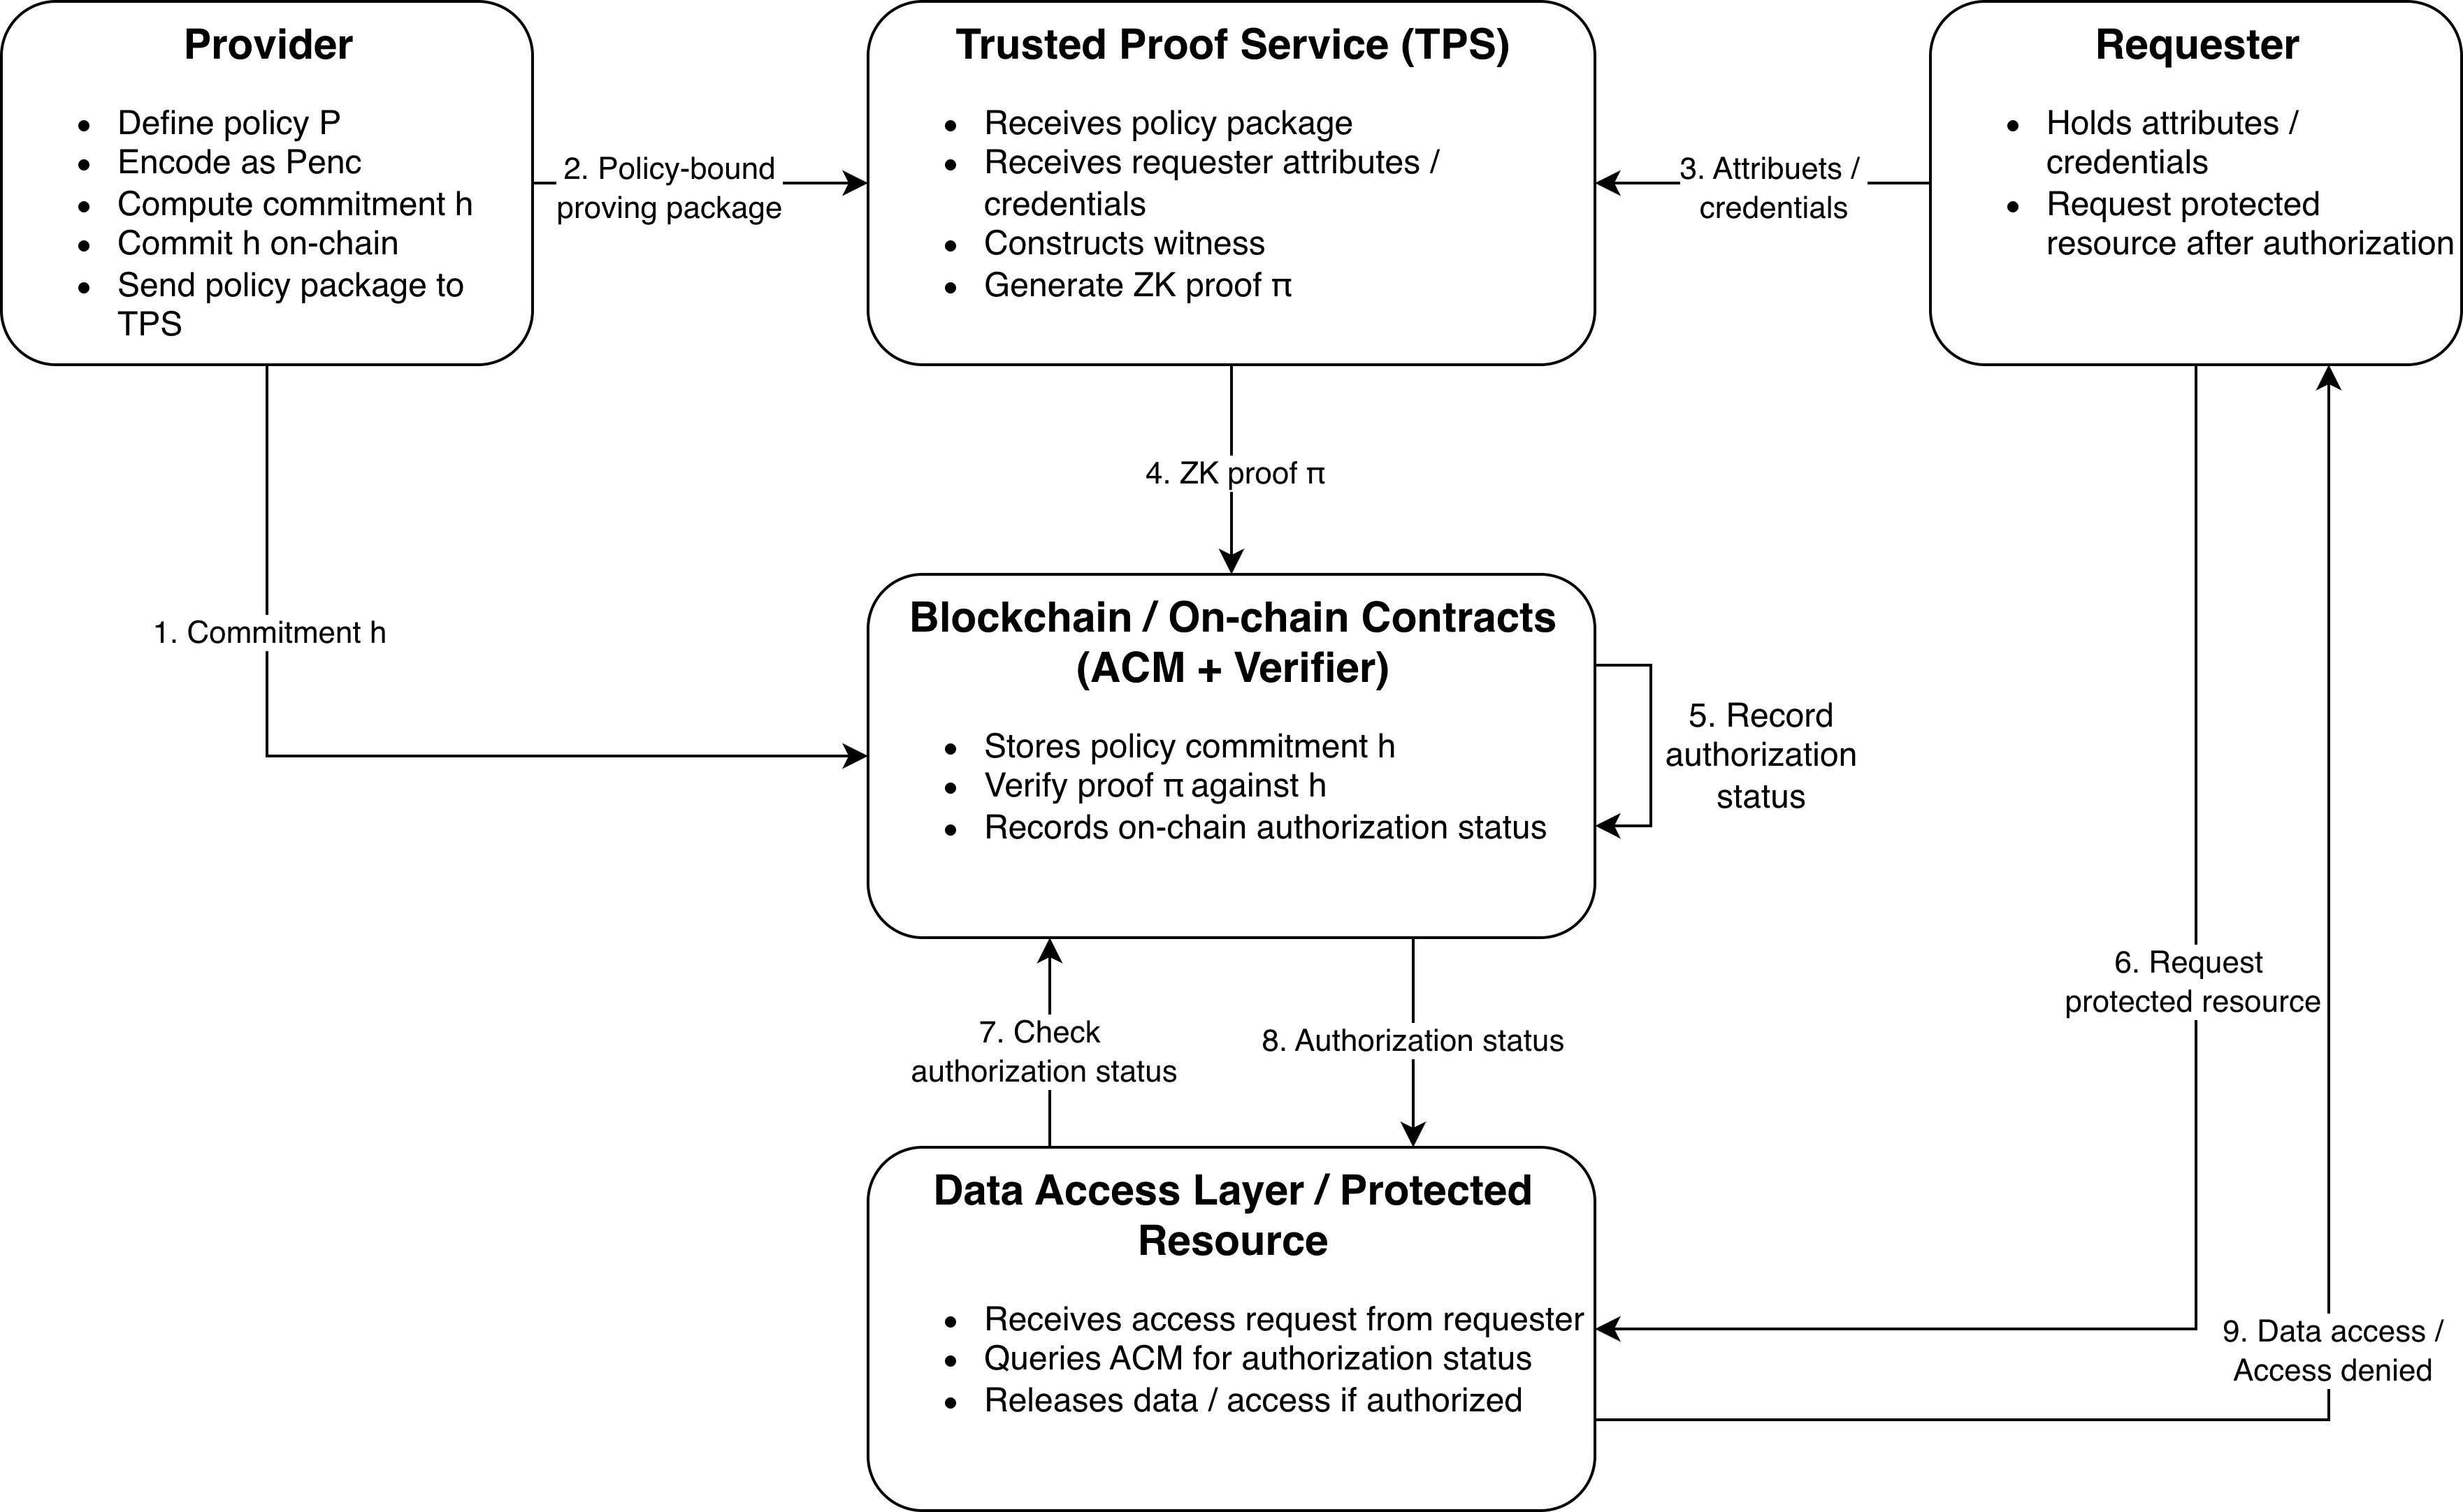
\includegraphics[width=0.9\textwidth]{PP-TPS.png}
	\caption{TPS-assisted policy-compliance workflow. The provider commits to the encoded policy on-chain and provisions proving material to the TPS (steps 1--2); the TPS constructs the witness from requester evidence and generates the proof (3--4); the ACM verifies the proof and records the outcome (5); the data access layer consults the recorded status to serve the requester (6--9).}
	\label{fig:tps-zkpi-workflow}
\end{figure}

\subsection{Policy Representation and Interpretation}

TPS-ZKPI represents heterogeneous Boolean-based consent policies in a fixed-length, circuit-friendly format.
This policy class is chosen for two reasons.
First, the targeted biomedical consent conditions---DUO-style data-use terms, disease-scope constraints, and institutional or ethics requirements---are categorical conditions combined with AND/OR/NOT, and conditions that are not natively Boolean, such as temporal validity or credential status, enter as externally attested predicate outcomes.
Second, a Boolean policy class admits a fixed-length encoding evaluated by a single reusable interpreter circuit, which keeps the verification interface policy-independent---a prerequisite for the privacy objectives evaluated later.
Let
\begin{equation}
	X = \{0,1\}^{N}, \qquad B = \{0,1\}^{M}
\end{equation}
denote the requester-attribute assignment space and the external-predicate assignment space, respectively.
The full assignment space is
\begin{equation}
	O = X \times B,
\end{equation}
where $a \in X$ encodes requester attributes and $b \in B$ encodes externally attested predicate outcomes, such as credential validity, ontology-linked checks, or obligation-related conditions.
Credential issuance, revocation, and attestation themselves remain external functions (Section~\ref{subsec:trust-model}): TPS-ZKPI consumes their outcomes as predicate bits and, where applicable, checks the associated auxiliary witnesses inside the proof relation.

Ontology-linked conditions are represented extensionally rather than through in-circuit ontology reasoning.
At encoding time, the provider expands an ontology concept into a whitelist of codes and commits the whitelist as a Merkle root among the policy's per-predicate parameters; in-circuit, the predicate check is a set-membership proof of the requested term against this root.
A disease-specific policy scoped to diabetes, for example, whitelists the ICD-10 diabetes subtree, whereas one scoped to type-1 diabetes whitelists only the type-1 codes.
Resolving subsumption at encoding time keeps ontology reasoning out of the circuit and preserves the policy-independent interface.

Consent policies are expressed as Boolean formulas over assignment bits:
\begin{equation}
	P ::= \mathit{atom} \mid (P \land P) \mid (P \lor P) \mid \neg P,\qquad
	\mathit{atom} ::= x_i \mid y_j .
\end{equation}
Here $x_i$ selects requester-attribute bit $a_i$ and $y_j$ selects external-predicate bit $b_j$.
For example, the consent condition ``the resource may be used for disease-specific research on diabetes, or for clinical care under approved clinical terms'' is expressed as $(x_1 \land y_1) \lor (x_2 \land y_2)$, where $x_1$ and $x_2$ flag the disease-specific-research and clinical-care purposes among the requester attributes, $y_1$ attests that the requested disease code lies in the committed diabetes whitelist, and $y_2$ attests that the requested clinical term lies in the approved clinical whitelist.
Each policy is compiled into a Reverse Polish Notation (RPN) program over operand tokens and Boolean operator tokens.
RPN linearizes arbitrarily nested formulas into a parenthesis-free token sequence that a stack machine evaluates in a single left-to-right pass with a fixed step count---a control structure that maps directly onto a fixed-size circuit and lets one interpreter serve all policies.
To support reusable verification, each program is padded to a fixed token length $L$:
\begin{equation}
	P_{\mathrm{enc}}= [t_{1},\ldots,t_{L}],
\end{equation}
together with an explicit program length $\ell \le L$ carried as a private witness.
The interpreter evaluates only the first $\ell$ tokens; padding positions beyond $\ell$ are inactive and leave the output unchanged.
The example policy above compiles to the token sequence $[x_1,\, y_1,\, \land,\, x_2,\, y_2,\, \land,\, \lor]$ with $\ell = 7$; the remaining $L-7$ positions are padding.
The implemented RC1 circuit uses $N=13$, $M=11$, and $L=\DEPTH=64$.
We denote the set of length-$L$ programs by $\mathsf{Prog}_{L}$.

The reusable policy interpreter is a zero-knowledge circuit
\begin{equation}
	C : \mathsf{Prog}_{L}\times \{0,\ldots,L\} \times O \rightarrow \{0,1\}.
\end{equation}
Given an encoded policy, its program length, and operand values, the interpreter evaluates the
RPN program using deterministic stack semantics and enforces well-formedness constraints inside the circuit.
The circuit outputs $1$ only if the requester evidence satisfies the encoded policy.
Well-formedness is enforced as hard constraints: for a program that violates the stack discipline, no satisfying witness exists and no proof can be generated.
An output of $0$ therefore indicates unsatisfied evidence for a well-formed program. The proved acceptance relation is the asserted case $C(P_{\mathrm{enc}},\ell,(a,b))=1$.

The fixed-length interpreter thus realizes the policy-independent interface motivated above, and supports policy evolution through different fixed-length policy programs.

\subsection{Commitment Binding and Proof Generation}

To bind each proof to a provider-defined hidden policy, the provider samples commitment randomness $r$ uniformly from the scalar field and computes
\begin{equation}
\begin{split}
	q &= \mathsf{H}_{\mathrm{pol}}(P_{\mathrm{enc}}),\\
	h &= \mathsf{Com}(P_{\mathrm{enc}},\ell; r)
	   = \mathsf{Poseidon}(q\parallel \ell\parallel r),
\end{split}
\end{equation}
where $q$ is the Poseidon-based digest of the fixed-length encoded policy, $\ell$ is the private program length, $r$ is the commitment randomness, and $h$ is the policy commitment stored on-chain.
The semantics of an encoded policy are determined by the pair $(P_{\mathrm{enc}},\ell)$, since $\ell$ identifies the active prefix of the padded token array.
Accordingly, the circuit supplies the same private value $\ell$ to both the commitment verifier and the policy interpreter.
Under the collision resistance of Poseidon, an accepting proof bound to $h$ cannot substitute a different program length and therefore cannot evaluate an alternative stack-consistent prefix of $P_{\mathrm{enc}}$.
Hiding is an explicit commitment assumption (Section~\ref{subsec:trust-model}) that relies on
high-entropy $r$ and the fixed-length encoding of $P_{\mathrm{enc}}$, which keeps the sponge input unambiguous.

For an access request, let
\begin{equation}
	\chi=(\mathit{id}_{\mathrm{req}},\mathit{id}_{\mathrm{res}},\nu),
	\qquad
	d_{\chi}=\mathsf{Poseidon}(\mathit{id}_{\mathrm{req}}\parallel
	\mathit{id}_{\mathrm{res}}\parallel\nu),
\end{equation}
where $\nu$ is a fresh session nonce.
The TPS constructs the private circuit witness
\begin{equation}
	w = (P_{\mathrm{enc}}, \ell, a, b, r, \omega, \chi),
\end{equation}
where $P_{\mathrm{enc}}$ is the encoded policy, $\ell$ is its program length, $a$ denotes requester attributes, $b$ denotes external predicate outcomes, $r$ is the commitment randomness, and $\omega$ denotes auxiliary witnesses for credential- or predicate-dependent checks.
The context tuple $\chi$ consists of private circuit inputs, while its digest $d_{\chi}$ is public.
The current public-signal vector is
\begin{equation}
	(1,h,\mathit{pp},d_{\chi},\tau),
\end{equation}
where $\mathit{pp}$ is a fixed-format commitment to the per-predicate parameters and $\tau$ is the request epoch used by the temporal checks.
Although the three components of $\chi$ are not separate Groth16 public inputs, the ACM receives them as transaction parameters in order to recompute $d_{\chi}$; they are therefore visible in transaction calldata.

For the compiled circuit, the Groth16~\cite{groth2016size} setup produces the common reference string as a proving key and a verification key, once for the shared circuit:
\begin{equation}
	(\mathit{pk}, \mathit{vk}) \leftarrow \mathsf{Setup}(C).
\end{equation}
The TPS generates a proof
\begin{equation}
	\pi \leftarrow \mathsf{Prove}\bigl(\mathit{pk}, w; (1,h,\mathit{pp},d_{\chi},\tau)\bigr).
\end{equation}
The proof certifies the conjunction that $C(P_{\mathrm{enc}},\ell,(a,b))=1$, $h=\mathsf{Com}(P_{\mathrm{enc}},\ell;r)$, $d_{\chi}=\mathsf{Poseidon}(\chi)$, and required external-predicate checks are internally consistent with respect to the supplied parameters and placeholder gadgets.
In the current implementation, the issuer-signature check among these gadgets is a hash-based placeholder (a Poseidon consistency check that provides no unforgeability), so attribute-origin binding is not an in-circuit guarantee; its scope and implications are treated in Sections~\ref{sec:problem} and~\ref{sec:discussion}.
Before verifying $\pi$, the ACM checks that the resource is governed by the stated policy, that $\tau$ is current, that the nonce has not been used for the same requester--resource context, and that the digest recomputed from the transaction parameters equals the public signal $d_{\chi}$.
Thus, within one ACM deployment, a proof generated for one requester identifier, resource, and nonce cannot be accepted under a different tuple.
The ACM then verifies $\pi$ against $\mathit{vk}$ and records the outcome of each request: a positive authorization outcome requires both a valid proof and an asserted output of $1$; otherwise the request is recorded as a denial.
The policy encoding, commitment randomness, requester attributes, credential witnesses, and auxiliary proof material are not posted on-chain.

\subsection{Transcript Normalization}

Zero-knowledge proofs hide private witness values, but surrounding
blockchain artifacts may still leak policy-dependent information. TPS-ZKPI therefore
normalizes the public transcript so that different policies induce fixed or tightly
bounded observable profiles. Table~\ref{tab:transcript-normalization}
summarizes the mechanisms.

\begin{table}[H]
	\centering
	\caption{Transcript-normalization mechanisms in TPS-ZKPI.}
	\label{tab:transcript-normalization} \footnotesize
	\begin{tabular}{p{0.24\linewidth}p{0.66\linewidth}}
		\hline
		\textbf{Artifact} & \textbf{Normalization mechanism}                                                   \\
		\hline
		Calldata          & Fixed verification interface and fixed-size proof/public-input encoding.           \\
		Logs              & Fixed event structure with constant topic and payload layout.                      \\
		Public parameters & Fixed-format handles instead of policy artifacts or credential witnesses.          \\
		Gas usage         & Policy-independent verifier logic and randomized gas padding toward fixed targets. \\
		\hline
	\end{tabular}
\end{table}

These mechanisms do not eliminate all public observability. Rather, they reduce policy-dependent variation in calldata, logs, public parameters, and gas-related behavior that could otherwise serve as a fingerprint for the metadata-only adversary defined in Section~\ref{sec:problem}.
TPS-ZKPI does not flatten all residual channels: timing between transactions, transaction ordering, mempool or broadcast patterns, and off-chain TPS communication remain outside the normalized public transcript.


% Top-level Evaluation chapter. \input this from the main manuscript.
% Requires in the preamble: \usepackage{booktabs} \usepackage{amsmath} \usepackage{amssymb} \usepackage{graphicx}
% If the main document uses a different graphics path for the figures, set it before \input.
\section{Experiments and Results}
\label{sec:eval}

We evaluate PCH, PI, and SPP (Section~\ref{subsec:privacy-objectives}) against a passive public-chain observer (Section~\ref{sec:eval-threat}).
The evidence comes from two attack families run on the same executions: a supervised attacker that tries to recover each hidden label from the on-chain observables, and an unsupervised attacker that asks whether the observables cluster along that label without seeing it.
Across the $45$ tasks, two meet the leakage criterion (one ICD-10 chapter and one nesting-depth contrast); both trace to the randomly drawn padding target, and the unsupervised attacker finds no natural grouping by the hidden labels beyond the same coincidence.
Table~\ref{tab:privacy-summary} summarizes the headline supervised verdicts across the three privacy objectives.
Beyond the privacy verdicts, we report the system's performance as a cost profile: per-transaction gas for commit and access (including the padding overhead), calldata sizes, circuit constraint count, and proving time, together with how circuit capacity, fixed-circuit policy complexity, and offline proof throughput scale.

% Sources of record (higher-AUC model per task; cross-checked against the JS verdicts):
%   PCH: python/results/supervised_analysis/pch_supervised_verdict.json
%   PI:  python/results/supervised_analysis/pi_supervised_verdict.json
%   SPP: python/results/supervised_analysis/spp_supervised_verdict.json
% (all 30 policy-disjoint seeds, deterministic per-seed RNG.)
% Dataset: Polygon Amoy, fixed circuit + commitment-only interface + access-gas padding.
\begin{table}[H]
  \centering
  \caption{Headline privacy results on the Polygon Amoy dataset. The supervised attacker
    uses 30 policy-disjoint seeds and a permutation test. A task passes unless both
    AUC$_{\text{mean}}>0.55$ and at least $50\%$ of seeds are significant.}
  \label{tab:privacy-summary}
  % Column widths sum to <1 so that the inter-column glue fits inside the text block.
  \begin{tabular}{p{0.16\linewidth}p{0.32\linewidth}p{0.42\linewidth}}
    \toprule
    Property & Hidden target & Headline supervised result \\
    \midrule
    PCH & DUO terms and ICD-10 chapters
        & 16 content-recovery tasks pass; DUO AUCs $0.493$--$0.526$, ICD AUCs $0.433$--$0.561$ \\
    PI & Related policy-pair identity
       & Overall AUC $0.514\pm0.022$, $7\%$ significant seeds \\
    SPP & Structure, predicate, parameter, and nesting-depth buckets
        & 28 pairwise contrasts pass; AUCs $0.483$--$0.629$, max $23\%$ significant seeds \\
    \bottomrule
  \end{tabular}
\end{table}

% Shared threat model for the three privacy experiments.
\subsection{Adversary and Observables}
\label{sec:eval-threat}

We consider the passive public-chain observer defined in Section~\ref{sec:problem}.
This adversary has unrestricted read access to the ledger and observes all transactions and events generated by TPS-ZKPI, but has no direct access to the plaintext policy or the witness.
Under the assumptions stated in Section~\ref{subsec:trust-model}, the zero-knowledge proof reveals no information beyond the public statement, and the hiding commitments conceal the committed policy.
These cryptographic protections do not, by themselves, prevent policy information from leaking through observable metadata.

We consider three adversary goals, one per privacy objective:
(i)~recover the policy's \emph{content} (PCH, Section~\ref{sec:eval-pch});
(ii)~distinguish two \emph{semantically related} policies (PI, Section~\ref{sec:eval-pi}); and
(iii)~recover the policy's \emph{structure or parameter sizes} (SPP, Section~\ref{sec:eval-spp}).

To evaluate attacks against these goals, we extract the following metadata features from each policy execution, consisting of a commit transaction followed by an access transaction:
%
\begin{itemize}
	\item \textbf{Gas:} \texttt{commitGasUsed}, \texttt{accessGasUsed}.
	\item \textbf{Calldata length:} \texttt{commitCalldataLength}, \texttt{accessCalldataLength}.
	\item \textbf{Proof size:} \texttt{proofSize}.
	\item \textbf{Event logs:} \texttt{commitLogsCount}, \texttt{commitLogsSize},
	      \texttt{accessLogsCount}, \texttt{accessLogsSize}.
\end{itemize}
%
The fixed circuit and commitment-only interface keep calldata length, proof size, and event-log counts and sizes constant across the evaluated policies.
These features remain in the attack pipeline but provide no variation for the attacks to exploit.
Any policy-dependent variation in the selected feature set must therefore occur in the two gas measurements (\texttt{commitGasUsed} and \texttt{accessGasUsed}).

% Shared methodology: supervised attack pipeline + unsupervised clustering cross-check.
\subsection{Attack Methodology}
\label{sec:eval-method}

We evaluate each privacy objective with a primary supervised attack and a complementary unsupervised cross-check.
The \emph{supervised} method trains classifiers on labeled data to predict hidden labels from the observables.
Performance is measured by AUC, with a chance baseline of $0.5$.
The \emph{unsupervised} method clusters the observables without using labels.
We evaluate agreement between the resulting clusters and the true labels using the Adjusted Rand Index (ARI) and Normalized Mutual Information (NMI).

We execute the generated policies on the \emph{Polygon~Amoy} testnet.
For each policy, a provider account submits the policy commitment using \texttt{commitPolicyWithGasPad}.
We then generate the Groth16 proof locally, acting as the TPS (Section~\ref{subsec:trust-model}).
A separate TPS account submits the access transaction using \texttt{requestAccessBoundWithGasPad}.
In the prototype, provider-to-TPS and requester-to-TPS exchanges are implemented as in-process calls and generate no additional on-chain artifacts.
We extract the observables defined in Section~\ref{sec:eval-threat} from the transaction receipts, calldata, and event logs.

\subsubsection{Supervised Attacks}
We evaluate each objective through binary classification \emph{tasks}, in which the attacker predicts a hidden label from the observables.
PCH tasks predict DUO-term presence or ICD-10 chapter membership (Section~\ref{sec:eval-pch}).
PI tasks distinguish between executions of two policies (Section~\ref{sec:eval-pi}).
SPP tasks distinguish between two categories of a structural or parameter property (Section~\ref{sec:eval-spp}).

For every task, we train two classifiers: logistic regression (LR) and random forest (RF), representing linear and non-linear models, respectively.
Each task is evaluated over \textbf{30 random seeds}, using the same protocol across PCH, PI, and SPP.

For each seed, we first randomly select one execution per policy to limit the influence of repeatedly executed policies on the AUC and its permutation test.
We then construct a \textbf{policy-disjoint $70/30$ train/test split}, ensuring that no policy appears in both sets.
Test AUC therefore measures attack performance on policies not seen during training.
Because policies are kept intact, exact per-class split proportions cannot always be achieved.
For each seed, we generate $512$ candidate splits and discard those that lack either class in the training or test set.
Among the valid candidates, we select the split that best approximates a $30\%$ test fraction within each class.

For each seed and classifier, we assess test AUC using a label-permutation test.
After training, we keep the test-set prediction scores fixed and randomly permute the test labels $R=500$ times.
We recompute AUC for each permutation to obtain its null distribution under no association between scores and labels.
The empirical $p$-value is
\begin{equation}
	p = \frac{k+1}{R+1},
	\label{eq:perm-p}
\end{equation}
where $k$ counts the permutations whose AUC is at least as large as the observed AUC.
The $+1$ correction prevents a zero $p$-value, with a minimum attainable value of $1/(R+1)$.
The result for a given seed and classifier is considered significant when $p<0.05$.

All tasks are binary, and the chance baseline for AUC is $0.5$ regardless of class balance.
Class imbalance may affect estimation uncertainty but does not change this baseline.

For each task, let $\mathrm{AUC}_s$ denote the test AUC for seed $s$, with $S=30$ seeds.
The results report the mean AUC and the AUC gap $G_{\mathrm{AUC}}$, defined as the mean absolute deviation from $0.5$:
\begin{equation}
	\mathrm{AUC}_{\text{mean}} = \frac{1}{S}\sum_{s=1}^{S}\mathrm{AUC}_s, \qquad
	G_{\mathrm{AUC}} = \frac{1}{S}\sum_{s=1}^{S}\left|\mathrm{AUC}_s-0.5\right|.
	\label{eq:auc-gap}
\end{equation}
Taking absolute deviations before averaging prevents values above and below $0.5$ from canceling.

The PASS/FAIL decision uses the mean AUC and the significant-seed fraction.
The latter is the fraction of seeds with $p<0.05$, reported as \%sig.
We classify each task as follows:
%
\begin{quote}
	\textbf{FAIL} if $\mathrm{AUC}_{\text{mean}}>0.55$ and at least $15$ of the $30$ seeds yield $p<0.05$.
	\textbf{PASS} otherwise.
\end{quote}
%
We refer to this rule as the \emph{leakage criterion}.
A PASS means that the evaluated attacks did not meet this criterion for the task.

The two conditions define an operational criterion based on effect size and consistency across splits.
With large test sets, even a small AUC increase above chance may be statistically significant.
The AUC threshold of $0.55$ prevents such small effects from triggering a FAIL solely on the basis of statistical significance.

The stability condition requires statistically significant results in at least half of the $30$ splits.
Because the splits overlap across seeds, the significant-seed fraction measures consistency across splits and is not interpreted as a combined $p$-value.

Because these thresholds are operational choices, we reapply the criterion over AUC thresholds of $0.52$--$0.60$ and significant-seed fractions of $0.3$--$0.7$.
At fractions of at least $0.5$, at most the two tasks discussed in the PCH and SPP result sections fail; lowering the fraction to $0.3$--$0.4$ adds at most two SPP contrasts, whereas raising it to $0.6$ yields none. No PI task fails under any of these threshold pairs.

In the evaluated run, the stability condition determines which tasks are flagged.
The AUC condition alone would flag four PCH and four SPP tasks.
In each objective, three of these tasks are significant in fewer than half of the splits.
The stability condition alone flags the same single task in each of PCH and SPP as the full leakage criterion.

In ten null reruns with policy-independent gas features, four contain a spurious PCH failure (a $3\%$ per-task frequency), while none produces an SPP failure.
We therefore examine the two observed failures in the corresponding result sections and keep them as FAIL.

The effectiveness of gas padding is assessed separately by the paired gas-padding ablation (Section~\ref{sec:eval-ablation}).
Using the same policies, features, splits, and classifiers, the attacks recover signal from the unpadded transcript, and that signal collapses after padding.
Thus, the leakage criterion summarizes residual attack performance, whereas the paired reduction provides the primary empirical evidence that padding suppresses the modeled gas channel.

The criterion is applied independently to LR and RF; a task fails if either classifier crosses both thresholds, and the result tables report the classifier with the higher mean AUC.

The classifiers receive all nine features stated in Section~\ref{sec:eval-threat}, including the seven that are constant by design.

\subsubsection{Unsupervised Clustering Attacks}
We run K-Means (with $K$ set to the number of classes, or $K=2$ for policy pairs) on the on-chain gas features, and score the recovered clusters against the true labels with ARI and NMI.
Values near $0$ mean the clusters carry no information about the hidden label; values near $1$ mean full leakage.

PCH clusters all executions globally, and SPP is clustered the same way on its $1{,}125$-execution view (Section~\ref{sec:eval-dataset}), once per annotation axis of Section~\ref{sec:eval-spp} with $K$ equal to that axis's bucket count.
At these sample sizes, ARI and NMI are read directly, each averaged over $20$ K-Means seeds.
To test whether an ARI exceeds chance, the cluster assignments are kept fixed, the labels are shuffled $200$ times, and $p_{\mathrm{ARI}}$ follows Equation~\eqref{eq:perm-p} with $R=200$, so its smallest attainable value is $1/201 \approx 0.005$.

For PI, clustering is scored per pair, so each side of a pair must contribute enough executions; this requires two safeguards.
First, the PI clustering analysis uses a dedicated set of \emph{balanced policy pairs} constructed from depth-layer executions (Section~\ref{sec:eval-dataset}).
We evaluate $127$ pairs, each containing $30$ executions per policy.
The policy pairs used in the supervised PI attack (Section~\ref{sec:eval-pi}) are unsuitable for per-pair clustering.
Most pairs contain only one execution per policy, while some contain $1$ execution for one policy and $30$ for the other.
These small or highly imbalanced samples make clustering scores unreliable indicators of policy distinguishability.
The supervised attack is unaffected, because it pools the executions of each pair type.
Second, NMI is \emph{permutation-debiased}. Even after balancing, each side of a pair holds only $30$ executions. At that scale NMI is inflated even without signal, whereas ARI is not (Section~\ref{sec:eval-nmi-sensitivity}), so ARI is read directly and NMI must be debiased.
The cluster assignments are computed once (K-Means does not see the labels) and the observed NMI is averaged over $20$ K-Means seeds; the pair labels are then shuffled $200$ times and the NMI recomputed against the fixed assignments on each shuffle, giving the null distribution of NMI under zero true signal.
The debiased NMI is the observed NMI minus the mean of this null distribution, and the empirical $p$-value $p_{\mathrm{NMI}}$ follows Equation~\eqref{eq:perm-p} with $R=200$, where $k$ counts the shuffles whose NMI meets or exceeds the observed value.
The cross-check flags a pair only if its debiased NMI is positive \emph{and} significant ($p_{\mathrm{NMI}}<0.05$).

% Dataset and corpus generation. \input from evaluation.tex after sec_threat_model.tex
% and before sec_methodology.tex. Numbers are of-record from
% experiments/data/polygonAmoy/executed_dataset.json and config.json (unpadded capture
% of 2026-10-15, v3.0.0-rc2 artifacts; see that directory's README.md).
\subsection{Dataset and Corpus Generation}
\label{sec:eval-dataset}

The PCH, PI, and SPP evaluations use policies from a dataset of $1{,}077$ distinct policies, run as $1{,}977$ on-chain executions on \emph{Polygon~Amoy}, each execution being one commit transaction followed by one access transaction.
The policies are produced by a deterministic generator with a fixed seed (\texttt{unified-decoupled-2026}), and the number of executions per policy follows from the two execution layers described below.
For reproducibility, the generator uses a deterministic test issuer to construct private credential witnesses for policies that require credential verification.

For each policy, the generator selects a set of DUO data-use terms and a logical form that combines them.
Five ontology-linked terms (Section~\ref{subsec:duo}) use code whitelists drawn from external vocabularies: DS uses ICD-10, RS uses the Ontology for Biomedical Investigations (OBI)~\cite{bandrowski2016ontology}, POA uses the Human Ancestry Ontology (HANCESTRO), GS uses ISO~3166 country codes, and CC uses SNOMED Clinical Terms (SNOMED~CT).
The other five terms (GRU, HMB, NMDS, GSO, NCU), which we call profile terms, are evaluated using signed claims from the requester's profile credential (Section~\ref{sec:design}).
The generator draws a fixed number of policies from each of six families defined by the terms and connectives they use: a single ontology-linked term, a single profile term, AND-only, OR-only, and mixed AND/OR combinations of several terms, and combinations of profile terms only.

Each policy contains one whitelist for each ontology-linked term it includes.
We draw a target whitelist size once per policy from $\{2, 4, 8, 12, 16, 20, 24, 32\}$, independently of its logical form.
This target applies to all whitelists in the policy.
If a selected scope contains fewer codes than the target, the corresponding whitelist contains only the available codes; this occurs in $8$ of the $2{,}000$ whitelists.
For analysis, we define a policy's whitelist size as the largest actual whitelist size within that policy.
The $147$ policies without an ontology-linked term are assigned a whitelist size of $0$.

For example, one generated policy combines the DUO terms RS (research-specific use) and DS (disease-specific use).
It requires the study design to belong to the OBI \emph{observational and comparative designs} family and the requested record to fall within the ICD-10 \emph{diseases of the circulatory system} chapter.
The two conditions are joined by \texttt{AND}, so access is granted only when both are satisfied.
Each condition is represented by a predicate that checks membership in a whitelist.
The RS predicate uses a whitelist of $8$ OBI study-design codes, while the DS predicate uses $8$ ICD-10 codes drawn from that chapter.
Both whitelist sizes fall within the ``medium'' parameter-size bucket in Table~\ref{tab:corpus}.

We execute the policies in two layers.
The \emph{coverage layer} executes $1{,}017$ distinct policies once each, spanning the content labels and the categories of policy structure and parameter size and allowing training and testing to use disjoint policies to assess generalization to unseen policies.
The \emph{depth layer} executes each of the $60$ policies in $30$ designed policy pairs $16$ times ($960$ executions), allowing training and testing to use different executions of the same policies to assess whether an observer can distinguish the policies within each pair.
For each request, the generator constructs requester evidence that either satisfies or violates the policy, so that the request is granted or denied.
In the coverage layer, granted and denied requests are balanced as closely as possible within each group of policies sharing a logical-form family and a set of DUO terms, to reduce associations between authorization outcomes and content labels.
Each depth-layer policy receives $8$ granted and $8$ denied requests.
All $1{,}977$ executions produced the planned authorization outcomes ($989$ granted and $988$ denied).

Every execution commits its own instance of its policy with fresh commitment randomness, so no two executions share a policy commitment, a parameter commitment, or an on-chain policy identifier.
The executions are submitted in an order shuffled with a fixed seed, independently of the policy labels, so the identifiers assigned in registration order carry no label information.
Every content label has at least $33$ policies, and Table~\ref{tab:corpus} summarizes the counts for each content label and each category of policy structure or parameter size.

% Source of record: experiments/data/polygonAmoy/executed_dataset.json (1077 policies,
%   1977 executions, generator seed "unified-decoupled-2026"; per-label policy and
%   execution counts: duoTermCodes, ontologyNamespace/ontologyValue, structureType,
%   nestingDepth, predicateCombo, paramType).
% DUO is multi-label: an execution carries every term its policy references, so the
% per-term rows overlap and their column sums exceed the corpus totals. ICD-10 rows
% cover only the policies with an ICD-10 scope (the DS policies), as the ICD-10 group
% heading states.
% Layout: groupings in pairs, side by side (DUO terms | ICD-10 chapters, then the SPP
% groupings two by two). Both label columns are as wide as and_or_mixed, so the two
% halves match. The empty 3em column 4 separates the halves; the rules under the group
% headings use \cmidrule without (l)/(r) trims, which latexdiff would break.
\begin{table}[htbp]
	\centering\footnotesize
	\caption{Composition of the shared policy corpus}
	\label{tab:corpus}
	\begin{tabular}{@{}w{l}{52pt}rr@{}w{l}{3em}@{}w{l}{52pt}rr@{}}
		\toprule
		Category      & Policies & Executions & & Category          & Policies & Executions \\
		\midrule
		\multicolumn{3}{@{}l@{}}{\textit{DUO data-use term} (multi-label)} & & \multicolumn{3}{@{}l@{}}{\textit{ICD-10 chapter} (DS policies)} \\
		\cmidrule{1-3}\cmidrule{5-7}
		GRU           & $302$    & $617$      & & ch0               & $44$     & $104$      \\
		DS            & $422$    & $677$      & & ch1               & $49$     & $94$       \\
		RS            & $412$    & $742$      & & ch2               & $33$     & $33$       \\
		POA           & $392$    & $737$      & & ch3               & $55$     & $100$       \\
		GS            & $382$    & $682$      & & ch4               & $41$     & $56$       \\
		CC            & $392$    & $632$      & & ch5               & $34$     & $49$       \\
		NCU           & $206$    & $506$      & & ch6               & $48$     & $63$      \\
		HMB           & $331$    & $661$      & & ch7               & $48$     & $48$       \\
		NMDS          & $237$    & $387$      & & ch8               & $33$     & $63$       \\
		GSO           & $236$    & $551$      & & ch9               & $37$     & $67$       \\
		              &          &            & & \textit{Subtotal} & $422$    & $677$      \\
		\addlinespace
		\multicolumn{3}{@{}l@{}}{\textit{SPP structureType}} & & \multicolumn{3}{@{}l@{}}{\textit{SPP nestingDepth}} \\
		\cmidrule{1-3}\cmidrule{5-7}
		trivial       & $130$    & $235$      & & flat              & $130$    & $235$      \\
		and\_only     & $294$    & $579$      & & shallow           & $210$    & $360$      \\
		or\_only      & $303$    & $513$      & & medium            & $335$    & $575$      \\
		and\_or\_mixed & $350$   & $650$      & & deep              & $402$    & $807$      \\
		\addlinespace
		\multicolumn{3}{@{}l@{}}{\textit{SPP predicateCombo}} & & \multicolumn{3}{@{}l@{}}{\textit{SPP paramType}} \\
		\cmidrule{1-3}\cmidrule{5-7}
		single        & $257$    & $497$      & & none              & $147$    & $297$      \\
		few           & $645$    & $1185$     & & small             & $232$    & $457$      \\
		many          & $175$    & $295$      & & medium            & $352$    & $547$      \\
		              &          &            & & large             & $346$    & $676$      \\
		\midrule
		\textbf{Corpus total} & $\mathbf{1077}$ & $\mathbf{1977}$ & & & & \\
		\bottomrule
	\end{tabular}

	\begin{tablenote}
		ICD-10 labels ch0--ch9 index the ten chapters used: A00--B99, C00--D48, D50--D89, E00--E90, F01--F99, G00--G99, I00--I99, J00--J99, K00--K93, and M00--M99.
	\end{tablenote}
\end{table}


The evaluated content labels cover ten DUO data-use terms and ten ICD-10 chapters (Table~\ref{tab:corpus}).
Evaluating every DUO term and individual ICD-10 code would require a substantially larger on-chain dataset.
We therefore evaluate DUO-term presence and ICD-10 chapter membership.


% Policy Content Hiding section body.
\subsection{Policy Content Hiding (PCH)}
\label{sec:eval-pch}

\noindent\textbf{Property.} PCH requires that the public-chain observer cannot recover the \emph{content} of a policy---its DUO data-use terms or the ICD-10 disease codes it references---better than chance.

\noindent\textbf{Scope of the labels.} The attack targets the ten DUO data-use terms of the corpus---general research use (GRU), disease-specific research (DS), research-specific restrictions (RS), population origins or ancestry research (POA), geographical restriction (GS), clinical care use (CC), non-commercial use (NCU), health or medical or biomedical research (HMB), no methods development (NMDS), and genetic studies only (GSO)---and disease codes aggregated to the ten ICD-10 chapters. This label restriction, its statistical-power rationale, and why category-level granularity is a conservative choice are detailed in Section~\ref{sec:eval-dataset}.

\noindent\textbf{Supervised attack.} Each DUO term defines a one-vs-rest binary task, on which we run the multi-seed pipeline of Section~\ref{sec:eval-method}.
Table~\ref{tab:pch-terms} reports the per-term verdicts: every DUO task stays below the $0.55$ AUC line, with mean AUC between $0.477$ and $0.540$; significant-seed fractions run up to $23\%$ (GRU), short of the $50\%$ gate, and with the AUC leg unmet none approaches the failure criterion.
The same pipeline applied to the ten ICD-10 chapters (one-vs-rest over the ICD-bearing rows only, median test $n{=}127$ per chapter; Table~\ref{tab:pch-icd10}) passes nine chapters and fails one.
Chapters ch1, ch2, and ch4 sit just above the AUC line (mean AUC $0.558$--$0.570$) but reproduce in at most $23\%$ of seeds, so they are boundary cases rather than stable channels.
Chapter ch5 (diseases of the nervous system) meets both legs: mean AUC $0.667$ with $53\%$ of seeds significant.
We report it as a FAIL of the criterion and examine below what the classifier separates.

\noindent\textbf{What the ch5 classifier separates.} The two gas features are the only non-constant observables, and the access-gas measurement is itself the sum of two parts: the target that the TPS draws uniformly at random from the padding band for that execution (Section~\ref{sec:design}) and the gas that the padded call consumes beyond it, which on Amoy is a near-constant $4{,}661$--$4{,}750$ gas for all $1773$ executions.
The observer sees only the sum, but the capture log records every target, so we can ask how much of the separability survives once the target is subtracted.
None does.
Over all $20$ PCH tasks the rank-based AUC of the access gas coincides with the AUC of the target alone to three decimals, and the AUC of the residual (gas minus target) lies between $0.47$ and $0.52$; for ch5 the gas and target AUCs are both $0.601$ and the residual AUC is $0.472$.
The $34$ ch5 policies simply drew targets whose mean lies $33{,}000$ gas above that of the other $388$ ICD-bearing policies, a $3.2\sigma$ deviation for a uniform draw of that size; because each coverage-layer policy is executed once, the $30$ seeds resample the same $34$ fixed draws, which is why the deviation reproduces across seeds.
Rerunning the of-record protocol unchanged on the residual in place of the access gas gives mean AUC $0.556$ with $10\%$ significant seeds (logistic regression) and $0.561$ with $17\%$ (random forest), a PASS; rerunning it on the target alone reproduces the FAIL ($0.686$, $63\%$).
The padded gas therefore carries a policy-independent random draw that happened to correlate with one chapter in this corpus, not information about the chapter; Section~\ref{sec:eval-method} quantifies how often the criterion produces such a false positive.



% Policy Indistinguishability section body.
\subsection{Policy Indistinguishability (PI)}
\label{sec:eval-pi}

PI evaluates whether an observer can identify which of two semantically related policies governs a given execution.
We evaluate PI using $30$ designed policy pairs, divided into three types with $10$ pairs each:
\begin{itemize}
	\item \texttt{semantic\_equivalent}: The two policies share the same logical form, consisting of the same DUO terms and Boolean structure, but differ in predicate parameter values, such as whitelist codes.
	\item \texttt{weak\_equivalent}: The two policies share the same set of DUO terms but differ in Boolean structure.
	\item \texttt{controlled\_difference}: The two policies differ in their sets of DUO terms. For each $k \in \{0,1,2,3,4\}$, we include two pairs whose policies differ in exactly $k$ of the four SPP dimensions (Section~\ref{sec:eval-spp}).
\end{itemize}
Each policy belongs to one pair, and which of its two policies is $P_0$ and which is $P_1$ is drawn at random.

The attacker knows both policies in a pair and can execute each policy to obtain labeled training examples.
Given the on-chain observables of an execution, the attacker predicts whether it was governed by $P_0$ or $P_1$.
For each random seed and policy pair, we split the executions of each policy equally between training and testing, separately for granted and denied outcomes.
We train LR and RF on the training executions and evaluate each classifier using test AUC.
Each execution commits a separate policy instance (Section~\ref{sec:eval-dataset}), so training and test executions never share a commitment.

For each pair type and classifier, we first average the test AUCs across the $10$ pairs for each seed.
To assess significance, we construct a null distribution of this average by repeatedly permuting the test labels within each pair, recomputing each pair's AUC, and averaging across pairs.
This yields one mean AUC and one permutation $p$-value per seed.
We then apply the leakage criterion (Section~\ref{sec:eval-method}) using the AUC averaged over the $30$ seeds and the fraction of seeds with $p<0.05$.

All three pair types are classified as PASS (Table~\ref{tab:pi-pairs}).
The highest mean AUC, $0.549$ for \texttt{semantic\_equivalent} pairs with RF, remains below the $0.55$ threshold, with $20\%$ of seeds significant.

% Source of record: experiments/results/supervised/pi_supervised_verdict.json
%   (higher-mean-AUC model per pair type; cross-checked against the JS pi_report.json verdict).
% Policy Indistinguishability -- within-pair supervised attack, 30 seeds; each seed tests
% half of the executions of every (policy, outcome) cell of every pair.
% Criterion: FAIL iff AUC_mean > 0.55 AND significant-seed fraction >= 0.5 (perm alpha=0.05,
% labels permuted within pairs). All three pair types gate.
% AUC gap = mean over seeds of |AUC_s - 0.5| from models.<m>.perSeed.auc.
% Positive control: positiveControl.models (synthetic N(0,1) feature shifted by 0.75 on P1);
% the column shows the model with the higher control mean AUC.
\begin{table}[htbp]
	\caption{Policy Indistinguishability: within-pair supervised attack over 30 seeds, by
		policy-pair type (higher-mean-AUC classifier per type).}
	\label{tab:pi-pairs}
	\centering\footnotesize
	\begin{tabular}{lcccccc}
		\toprule
		Pair type              & Pairs & AUC (mean\,$\pm$\,std) & AUC gap (mean) & \%sig  & med $n$ & Control AUC (\%sig) \\
		\midrule
		semantic\_equivalent   & $10$  & $0.549 \pm 0.035$      & $0.052$        & $20\%$ & $160$   & $0.649$ ($93\%$)    \\
		weak\_equivalent       & $10$  & $0.520 \pm 0.045$      & $0.042$        & $7\%$  & $160$   & $0.611$ ($63\%$)    \\
		controlled\_difference & $10$  & $0.478 \pm 0.026$      & $0.028$        & $0\%$  & $160$   & $0.621$ ($87\%$)    \\
		\bottomrule
	\end{tabular}

	\begin{tablenote}
		med $n$: median test-set size over seeds, summed over the $10$ pairs of a type ($16$ of the $32$ executions of each pair). Control: the attack with one added synthetic feature drawn from a standard normal distribution and shifted by $0.75$ for $P_1$; shown for the classifier with the higher control mean AUC (LR for all three types).
	\end{tablenote}
\end{table}

% Structure & Parameter Privacy section body.
\subsection{Structure and Parameter Privacy (SPP)}
\label{sec:eval-spp}

To evaluate SPP, we annotate each policy along four dimensions that capture the structural and parametric properties described in Section~\ref{subsec:privacy-objectives}.
The four dimensions are logical structure type (\texttt{structureType}), predicate count (\texttt{predicateCombo}), parameter size (\texttt{paramType}), and nesting depth (\texttt{nestingDepth}).
Each dimension is divided into discrete categories or value ranges.
Specifically, \texttt{structureType} classifies the logical form joining the DUO terms (Section~\ref{sec:eval-dataset}) into four categories: \texttt{trivial} (a single term with no Boolean connective, e.g.\ policy logic \texttt{"DS"}), \texttt{and\_only}, \texttt{or\_only}, and \texttt{and\_or\_mixed}.
\texttt{predicateCombo} groups policies by predicate-namespace count into \texttt{single} ($1$), \texttt{few} ($2$--$3$), and \texttt{many} ($\ge 4$);
\texttt{paramType} groups policies by whitelist size into \texttt{none} (no whitelist), \texttt{small} ($1$--$4$), \texttt{medium} ($5$--$16$), and \texttt{large} ($\ge 17$);
\texttt{nestingDepth} groups policies by the maximum nesting depth of the normalized expression into \texttt{flat} ($\le 1$), \texttt{shallow} ($2$), \texttt{medium} ($3$), and \texttt{deep} ($\ge 4$).
In the normalized expression, each term is joined by AND to the predicate that checks it (e.g.\ \texttt{"DS"} becomes \texttt{(DS \& P[ICD10])}).
The policy counts for each category in the dataset are listed in Table~\ref{tab:corpus}.

Each pair of categories within a dimension defines a binary classification task.
Using the observables, the attacker predicts which of the two categories the executed policy belongs to.

Table~\ref{tab:spp-contrasts} reports the results for all pairwise classification tasks.
For most tasks, mean AUCs are close to the chance level of $0.5$, ranging from $0.490$ to $0.546$.
The \texttt{structureType} task \texttt{trivial}/\texttt{or\_only} and the \texttt{nestingDepth} task \texttt{flat}/\texttt{medium} both have a mean AUC of $0.559$.
Although these values exceed the $0.55$ threshold, their significant-seed fractions are $27\%$ and $37\%$, below the $50\%$ threshold, so all $21$ tasks are classified as PASS.

% Source of record: experiments/results/supervised/spp_supervised_verdict.json
%   (higher-AUC model per contrast; cross-checked against the JS report.json verdict).
% Structure & Parameter Privacy — supervised attack, multi-seed (30 policy-disjoint seeds).
% AUC is the higher of logistic regression / random forest per contrast (the
% "stronger attacker" leg used for gating).
% Criterion: FAIL iff AUC_mean > 0.55 AND significant-seed fraction >= 0.5 (perm alpha=0.05).
% structureType has a 5th category, "trivial": single-atom policies with no boolean
% connective (e.g. logicOriginal "GR" or "DS"), previously misclassified as and_only.
% p_perm and the AUC-gap std are not emitted by the Python pipeline; %sig (the gating
% significant-seed fraction) is retained, so the table now runs five columns.
\begin{table}[H]
  \caption{Structure \& Parameter Privacy: 28 pairwise contrasts across four annotation
    axes, each over 30 policy-disjoint seeds. AUC is the higher-scoring of logistic
    regression and random forest per contrast (the stronger-attacker classifier used for
    the verdict). Every contrast passes: the four contrasts whose AUC exceeds $0.55$---all
    separating the tiny \texttt{none}-predicate or \texttt{none}-parameter class from a
    populated one---reach at most $20\%$ significant seeds, far short of the $50\%$ gate.}
  \label{tab:spp-contrasts}
  \centering\footnotesize
  \begin{tabular}{lcccc}
    \toprule
    Contrast & AUC (mean\,$\pm$\,std) & AUC gap (mean) & \%sig & med $n$ \\
    \midrule
    \multicolumn{5}{l}{\textit{structureType}} \\
    trivial / or\_only                & $0.539 \pm 0.043$ & $0.042$ & $23\%$ & $156$ \\
    trivial / and\_only                & $0.535 \pm 0.044$ & $0.042$ & $3\%$  & $78$  \\
    trivial / negation\_heavy          & $0.508 \pm 0.046$ & $0.034$ & $3\%$  & $138$ \\
    trivial / and\_or\_mixed           & $0.533 \pm 0.047$ & $0.047$ & $13\%$ & $108$ \\
    and\_only / or\_only              & $0.531 \pm 0.050$ & $0.045$ & $10\%$ & $140$ \\
    or\_only / negation\_heavy        & $0.520 \pm 0.036$ & $0.033$ & $10\%$ & $202$ \\
    or\_only / and\_or\_mixed         & $0.489 \pm 0.026$ & $0.024$ & $0\%$  & $170$ \\
    and\_only / negation\_heavy       & $0.512 \pm 0.041$ & $0.035$ & $3\%$  & $125$ \\
    and\_only / and\_or\_mixed        & $0.513 \pm 0.059$ & $0.051$ & $0\%$  & $95$  \\
    negation\_heavy / and\_or\_mixed  & $0.516 \pm 0.044$ & $0.038$ & $7\%$  & $155$ \\
    \midrule
    \multicolumn{5}{l}{\textit{predicateCombo}} \\
    none / single   & $0.582 \pm 0.129$ & $0.130$ & $0\%$  & $74$  \\
    none / few      & $0.629 \pm 0.099$ & $0.138$ & $20\%$ & $216$ \\
    none / many     & $0.617 \pm 0.106$ & $0.119$ & $13\%$ & $59$  \\
    single / few    & $0.515 \pm 0.036$ & $0.031$ & $7\%$  & $284$ \\
    single / many   & $0.500 \pm 0.039$ & $0.029$ & $0\%$  & $127$ \\
    few / many      & $0.483 \pm 0.029$ & $0.026$ & $0\%$  & $269$ \\
    \midrule
    \multicolumn{5}{l}{\textit{paramType}} \\
    none / small    & $0.543 \pm 0.115$ & $0.096$ & $3\%$  & $66$  \\
    none / medium   & $0.612 \pm 0.080$ & $0.125$ & $17\%$ & $204$ \\
    none / large    & $0.545 \pm 0.093$ & $0.086$ & $0\%$  & $78$  \\
    small / medium  & $0.521 \pm 0.033$ & $0.030$ & $10\%$ & $263$ \\
    small / large   & $0.513 \pm 0.048$ & $0.036$ & $0\%$  & $138$ \\
    medium / large  & $0.486 \pm 0.023$ & $0.022$ & $0\%$  & $277$ \\
    \midrule
    \multicolumn{5}{l}{\textit{nestingDepth}} \\
    flat / shallow   & $0.522 \pm 0.040$ & $0.037$ & $13\%$ & $228$ \\
    flat / medium    & $0.499 \pm 0.043$ & $0.036$ & $3\%$  & $106$ \\
    flat / deep      & $0.490 \pm 0.033$ & $0.030$ & $0\%$  & $103$ \\
    shallow / medium & $0.511 \pm 0.028$ & $0.023$ & $0\%$  & $240$ \\
    shallow / deep   & $0.492 \pm 0.032$ & $0.026$ & $0\%$  & $237$ \\
    medium / deep    & $0.492 \pm 0.040$ & $0.032$ & $0\%$  & $115$ \\
    \bottomrule
  \end{tabular}
\end{table}

% Cross-objective unsupervised clustering section (consolidated view + PI rebalancing).
\subsection{Unsupervised Clustering: A Label-Free Cross-Check}
\label{sec:eval-clustering}
The clustering attacker stated in Section~\ref{sec:eval-method} tests whether the on-chain observables group by a hidden label without access to that label.
Table~\ref{tab:clustering-summary} summarizes the clustering results across the three privacy objectives.

ARI stays within $\pm 0.003$ for every PCH, PI, and SPP target except the SPP \texttt{nestingDepth}, indicating little agreement between the clusters and the hidden labels.
The PCH and SPP NMI values are below $0.03$, and apart from \texttt{nestingDepth} none is significant under the label-permutation test ($p_{\mathrm{NMI}}\ge 0.08$).
For PI, $6$ of the $127$ pairs ($5\%$) have $p_{\mathrm{NMI}}<0.05$, consistent with the nominal $5\%$ level.


For \texttt{nestingDepth}, the ARI and NMI are small but statistically significant under the label-permutation test reported in Table~\ref{tab:clustering-summary}.
To investigate this association, we repeat clustering on the same executions, retaining commit gas and replacing access gas with the residual defined in Equation~\eqref{eq:gas-decomp}.
The nesting-depth ARI then falls to $-0.0004$, and neither ARI nor NMI remains statistically significant ($p_{\mathrm{ARI}}=0.60$, $p_{\mathrm{NMI}}=0.69$).
Together with the diagnostic for the \texttt{medium}/\texttt{deep} contrast in Section~\ref{sec:eval-spp}, this result is consistent with a chance association between the randomly drawn padding targets and nesting depth in the evaluated dataset.
However, the residual analysis yields a small but nominally significant ARI for \texttt{paramType} ($0.0026$, $p_{\mathrm{ARI}}=0.04$), whose NMI is not significant ($p_{\mathrm{NMI}}=0.09$).
These findings provide complementary evidence to the supervised results on the same dataset.

% Sources of record:
%   PCH-DUO:   experiments/results/clustering/pch/pch_global_duo_clustering.csv
%              (global, all 1773 executions, no layering; K = 10 primary DUO terms)
%   PCH-ICD10: experiments/results/clustering/pch/pch_global_icd10_clustering.csv
%              (global, all 770 executions of the DS policies, which carry the ICD-10 scope; no layering)
%   PI:        experiments/results/clustering/pi/pi_balanced_debiased.csv
%              (127 balanced 30v30 pairs; observed means)
%   SPP:       experiments/results/clustering/spp/spp_clustering_summary.csv
%              (raw field names logicStructure/predicateCount/setSize map to the
%               supervised axes structureType/predicateCombo/paramType)
% Dataset: experiments/data/polygonAmoy/ (same executions as the supervised verdicts).
% p_ARI / p_NMI are the permutation p-values of the ensemble ARI / NMI (ari_p_value / nmi_p_value).
% Residual diagnostics (cited in sec_clustering.tex, not in this table):
%   experiments/results/supervised/pad_residual_diagnostic.json
%   experiments.spp.clustering.{nestingDepth,paramType}.residual
\begin{table}[htbp]
	\centering
	\caption{Unsupervised clustering attack (K-Means, $K$ = number of classes, $K=2$ for
		pairs) on the on-chain gas features.}
	\label{tab:clustering-summary}
	\footnotesize
	\setlength{\tabcolsep}{4pt}
	\begin{tabular}{@{}llcccccc@{}}
		\toprule
		Objective & Target                   & $n$    & \#cls. & ARI       & $p_{\mathrm{ARI}}$ & NMI      & $p_{\mathrm{NMI}}$ \\
		\midrule
		PCH       & DUO terms                & $1773$ & $10$   & $0.0000$  & $0.48$             & $0.0109$ & $0.41$             \\
		PCH       & ICD-10 chapters          & $770$  & $10$   & $0.0021$  & $0.06$             & $0.0281$ & $0.08$             \\
		PI        & policy pairs ($30$v$30$) & $127$  & $2$    & $0.0020$  & ---                & $0.0139$ & ---                \\
		SPP       & \texttt{structureType}   & $1125$ & $4$    & $0.0004$  & $0.33$             & $0.0034$ & $0.34$             \\
		SPP       & \texttt{predicateCombo}  & $1125$ & $3$    & $-0.0005$ & $0.58$             & $0.0015$ & $0.51$             \\
		SPP       & \texttt{paramType}       & $1125$ & $4$    & $-0.0000$ & $0.49$             & $0.0030$ & $0.43$             \\
		SPP       & \texttt{nestingDepth}    & $1125$ & $4$    & $0.0071$  & $<0.01$            & $0.0088$ & $<0.01$            \\
		\bottomrule
	\end{tabular}

	\begin{tablenote}
		For PI, ARI and NMI are means across the $127$ balanced policy pairs.
		Each pair is clustered and tested separately, so no single $p$-value applies to these means (---).
	\end{tablenote}
\end{table}



% Sample-size sensitivity of NMI under a null where all classes are i.i.d.
% Source of record: experiments/analysis/clustering/nmi_null_simulation.py (seed 20260923)
%   -> experiments/results/clustering/null/nmi_null_simulation.{json,md}; T=1000 per row.
% Supports the clustering cross-check (Section~\ref{sec:eval-clustering}): explains why
% small-sample NMI can be elevated even with no class-distinguishing signal.
\section{Sample-Size Sensitivity of NMI}
\label{app:nmi-sensitivity}

The clustering cross-check reads ARI directly but debiases the NMI of the balanced PI pairs (Section~\ref{sec:eval-method}).
To examine that choice, we quantify how \emph{finite-sample effects} alone can inflate NMI
even when there is \emph{no} discriminative signal, using an idealized null in which all
classes are statistically indistinguishable.

We sample every class from the \emph{same} distribution, $z_{i}\sim\mathcal{N}(0,I_{d})$ for all classes, where $I_d$ is the $d$-dimensional identity covariance and $d=2$ matches the two gas features the clustering uses.
Since no class carries class-specific information, a clustering algorithm should not recover class membership,
and both NMI and ARI should concentrate around $0$ as the sample size grows.

For each configuration we run $T=1000$ independent trials.
In each trial we
(i)~generate $G$ classes with $n$ i.i.d.\ samples per class from $\mathcal{N}(0,I_d)$, for $n_{\mathrm{tot}}=Gn$ samples in total, assigning each sample a class label by construction order (these labels are independent of the sample values, since all classes share one distribution),
(ii)~standardize the pooled data and apply K-Means with $K=G$ and ten initializations, as in the evaluation, and
(iii)~score the predicted assignments against these assigned class labels with NMI and ARI.
We vary $n$ while holding $G$ fixed, and report the trial means $\overline{\mathrm{NMI}}$ and $\overline{\mathrm{ARI}}$.
We consider a \textbf{PI-like} binary structure ($G=2$, $n\in\{3,10,50,100\}$), a five-class structure ($G=5$, $n\in\{3,10,100\}$), and a ten-class structure ($G=10$, $n\in\{3,10,77\}$) together with the observed ICD-10 chapter sizes ($49$--$135$ executions per chapter, $n_{\mathrm{tot}}=770$).

Table~\ref{tab:nmi-sample-size-sensitivity} shows that, although all classes are indistinguishable by construction, \textbf{NMI is noticeably positive at very small $n$ but collapses toward zero as $n$ grows}, whereas \textbf{ARI stays near zero throughout}.
For the binary structure, $\overline{\mathrm{NMI}}$ falls from $0.2074$ at $n=3$ ($n_{\mathrm{tot}}=6$) to $0.0420$ at $n=10$, and to $0.0072$/$0.0034$ at $n=50$/$100$.
The same trend holds with more classes, at a higher level for every $n$: with five classes $\overline{\mathrm{NMI}}$ goes from $0.4152$ ($n=3$) to $0.0102$ ($n=100$), and with ten classes from $0.5346$ ($n=3$) to $0.0239$ ($n=77$).
For the observed ICD-10 chapter sizes, a separate null run that averages each trial over $20$ K-Means seeds, as the evaluation does, gives a null NMI with mean $0.0246$ and $95$th percentile $0.0302$; the observed ICD-10 NMI of $0.0281$ is reached in $145$ of $1000$ null trials ($p=0.15$).

\begin{table}[htbp]
	\centering
	\caption{Sample-size sensitivity of NMI and ARI under the null hypothesis where all
		classes are i.i.d.\ sampled from $\mathcal{N}(0,I_d)$.}
	\label{tab:nmi-sample-size-sensitivity}
	\begin{tabular*}{0.54\linewidth}{@{\extracolsep{\fill}}rrrr@{}}
		\toprule
		$n$ (per class) & $n_{\mathrm{tot}}$ & $\overline{\mathrm{NMI}}$ & $\overline{\mathrm{ARI}}$ \\
		\midrule
		\multicolumn{4}{@{}l}{\textit{Two classes (as in a PI pair)}} \\
		$3$       & $6$   & $0.2074$ & $0.0127$  \\
		$10$      & $20$  & $0.0420$ & $0.0008$  \\
		$50$      & $100$ & $0.0072$ & $-0.0003$ \\
		$100$     & $200$ & $0.0034$ & $-0.0004$ \\
		\addlinespace
		\multicolumn{4}{@{}l}{\textit{Five classes}} \\
		$3$       & $15$  & $0.4152$ & $-0.0034$ \\
		$10$      & $50$  & $0.1226$ & $0.0003$  \\
		$100$     & $500$ & $0.0102$ & $-0.0000$ \\
		\addlinespace
		\multicolumn{4}{@{}l}{\textit{Ten classes (as the DUO and ICD-10 targets)}} \\
		$3$       & $30$  & $0.5346$ & $-0.0009$ \\
		$10$      & $100$ & $0.2087$ & $0.0003$  \\
		$77$      & $770$ & $0.0239$ & $-0.0001$ \\
		\addlinespace
		\multicolumn{4}{@{}l}{\textit{Ten classes, observed ICD-10 chapter sizes}} \\
		$49$--$135$ & $770$ & $0.0244$ & $-0.0001$ \\
		\bottomrule
	\end{tabular*}

	\begin{tablenote}
		$T=1000$ trials per row, one K-Means fit with ten initializations per trial; $n_{\mathrm{tot}}$ is the total sample size.
		For the observed ICD-10 chapter sizes, the text also reports a separate run that averages each trial over $20$ K-Means seeds, as the evaluation does.
	\end{tablenote}
\end{table}

% Gas-padding ablation / mechanism attribution.
\subsection{Gas-Padding Ablation}
\label{sec:eval-ablation}

Only the gas measurements vary across policies within the selected feature set (Section~\ref{sec:eval-threat}).
We therefore use the ablation to assess how randomized gas padding affects the attackers' ability to infer hidden policy information.

We compare two configurations, B1 and B2, that differ only in whether randomized gas padding is enabled.
Both use the fixed circuit, commitment-only interface, and TPS execution profile.
We evaluate both configurations on the same policy subset, selected deterministically from the evaluation corpus.
B1 disables padding for both policy commitment and access transactions, whereas B2 enables it for both.
B2 uses the same protection configuration as the PCH, PI, and SPP evaluations (Sections~\ref{sec:eval-pch}, \ref{sec:eval-pi}, and~\ref{sec:eval-spp}).

To quantify the effect of padding on attack performance, we compare the absolute AUC deviation from $0.5$ under B1 and B2.
For each paired train/test split $s$, we define
%
\begin{equation}
	\Delta_{\text{leak},s} =
	|\mathrm{AUC}_{\mathrm{B1},s} - 0.5| -
	|\mathrm{AUC}_{\mathrm{B2},s} - 0.5|,
	\label{eq:delta-leak}
\end{equation}
%
where positive values mean padding moved the attacker closer to chance.

For each task, we compute $\Delta_{\text{leak},s}$ over $30$ paired train/test splits, one for each random seed, using the same test policies for B1 and B2 in each split.
We report the mean $\Delta_{\text{leak}}$ with a $95\%$ percentile-bootstrap confidence interval (CI), obtained by resampling the split-level differences.
Table~\ref{tab:ablation-gas-padding} summarizes the results, and Figure~\ref{fig:ablation-paired} visualizes the comparison between B1 and B2.

% Source of record (supervised rows + counts):
%   python/results/supervised_analysis/gas_padding_supervised_deltaLeakage.csv
%   (metadata: gas_padding_supervised_metadata.json)
% B1 = unpadded gas transcript; B2 = deployed randomized access-gas padding.
% Effect = |AUC_B1-0.5| - |AUC_B2-0.5|; 95% repeated-split stability interval over
% 30 paired seeds (nonContemporaneous B1/B2 profiles).
% This table is ILLUSTRATIVE: the four supervised rows are representative contrasts whose
% stability interval of dLeak excludes zero (genuine reduction). They are NOT the full set.
% The full per-contrast distribution (all 49 rf + 49 lr contrasts, colored by dLeak CI
% sign) is the primary evidence and lives in Fig. fig:ablation-paired. Full-set counts:
%   RF: 36 reduce / 13 no-eff / 0 neg;  LR: 36 reduce / 11 no-eff / 2 neg.
% The unsupervised-ARI and gas-cost rows below are retained from the deployed on-chain
% ablation run (experiments/ablation/gas_padding/...); they are not part of the Python
% supervised recompute.
\begin{table}[H]
  \centering
  \caption{Gas-padding ablation on Polygon Amoy: representative contrasts illustrating the
    padding effect. B1 (no gas padding) and B2 (deployed, randomized access-gas padding) are
    aligned on the same policy set. Supervised AUC is the random-forest score (the stronger
    of the two classifiers here; see Section~\ref{sec:eval-method}); clustering reports K-Means ARI.
    $\Delta_{\text{leak}}>0$ (defined in the text) means padding moved the attacker toward chance,
    reported as the mean with a $95\%$ stability interval over $30$ paired splits. Each supervised
    row is, per experiment, the largest-signal contrast whose $\Delta_{\text{leak}}$ interval excludes
    zero (two for SPP), chosen to avoid cherry-picking. The full per-contrast distribution is in
    Figure~\ref{fig:ablation-paired}.}
  \label{tab:ablation-gas-padding}
  \begin{tabular}{lp{0.34\linewidth}cc}
    \toprule
    Attack & Target & B1 (unpad.) & B2 (pad.) \\
    \midrule
    \multicolumn{4}{l}{\textbf{Supervised} (RF AUC; $\Delta_{\text{leak}}$ with $95\%$ interval)} \\
    SPP   & \texttt{nestingDepth flat/deep}   & $0.847$ & $0.553$ \\
          & \quad $\Delta_{\text{leak}}=0.280$ CI$[0.254,0.304]$ & & \\
    SPP   & \texttt{structureType trivial/negation\_heavy} & $0.843$ & $0.524$ \\
          & \quad $\Delta_{\text{leak}}=0.276$ CI$[0.248,0.301]$ & & \\
    PCH   & ICD ch8                          & $0.918$ & $0.410$ \\
          & \quad $\Delta_{\text{leak}}=0.327$ CI$[0.302,0.349]$ & & \\
    PI    & \texttt{semantic\_equivalent}\,$^{\dagger}$  & $0.361$ & $0.500$ \\
          & \quad $\Delta_{\text{leak}}=0.140$ CI$[0.084,0.205]$ & & \\
    \midrule
    \multicolumn{4}{l}{\textbf{Unsupervised} (K-Means ARI)} \\
    PCH   & ICD-10 chapter                   & $0.064$ & $-0.005$ \\
    SPP   & logic structure                  & $0.043$ & $-0.001$ \\
    SPP   & predicate count                  & $0.054$ & $0.001$  \\
    \midrule
    \multicolumn{4}{l}{\textbf{Gas cost} (mean, B1 $\to$ B2)} \\
    \multicolumn{2}{l}{Commit gas} & $216{,}562$ & $303{,}556$ ($+40.2\%$) \\
    \multicolumn{2}{l}{Access gas} & $546{,}876$ & $753{,}310$ ($+37.7\%$) \\
    \bottomrule
  \end{tabular}

  \noindent{\footnotesize{$^{\dagger}$ B1 sits below $0.5$: the unpadded attacker separates the
  pair in the inverted direction (still $0.14$ from chance). $\Delta_{\text{leak}}$ is defined on
  $|\mathrm{AUC}-0.5|$.}}
\end{table}


Figure~\ref{fig:ablation-paired} shows each supervised task as one point, giving $20$ PCH, $21$ SPP, and $4$ PI tasks per panel.
The horizontal and vertical axes give the absolute deviation from $0.5$ of the mean AUC over the $30$ splits under B1 and B2, respectively.
A mean AUC below $0.5$ therefore also counts as a deviation.
Points below the diagonal indicate that padding moves the mean AUC closer to chance.
Both panels show the same pattern. Tasks with large deviations under B1 move well below the diagonal, whereas tasks near chance under B1 stay in the lower-left corner on both sides of the diagonal.

For RF, $21$ tasks have mean AUCs that deviate from $0.5$ by more than $0.15$ under B1.
Under B2, all $21$ fall below this level, and their median deviation is $0.037$, comparable to $0.041$ for the remaining $24$ tasks.
The confidence intervals for $\Delta_{\text{leak}}$ lie entirely above zero for all $21$ tasks, supporting a reduction in deviation from chance.
Across all tasks, the median deviation decreases from $0.137$ under B1 to $0.038$ under B2.
LR shows a similar pattern.
All $19$ tasks with deviations above $0.15$ under B1 fall below this level under B2, and the median deviation across all tasks decreases from $0.111$ to $0.037$.



Tasks already close to chance under B1 show no consistent change after padding.
For RF, $12$ tasks have CIs for $\Delta_{\text{leak}}$ that include zero, and their B1 deviations are at most $0.095$.
Another $6$ tasks have CIs entirely below zero, indicating increased deviation from chance, although their B1 deviations are at most $0.045$.
The largest increase occurs for ch5, whose mean AUC changes from $0.455$ under B1 to $0.631$ under B2.
Such increases may reflect chance associations between the randomly drawn padding targets and the hidden labels.
Related diagnostic analyses for ch5 and the \texttt{nestingDepth} comparison \texttt{medium}/\texttt{deep} illustrate this effect (Sections~\ref{sec:eval-pch} and~\ref{sec:eval-spp}).

\begin{figure}[htbp]
	\centering
	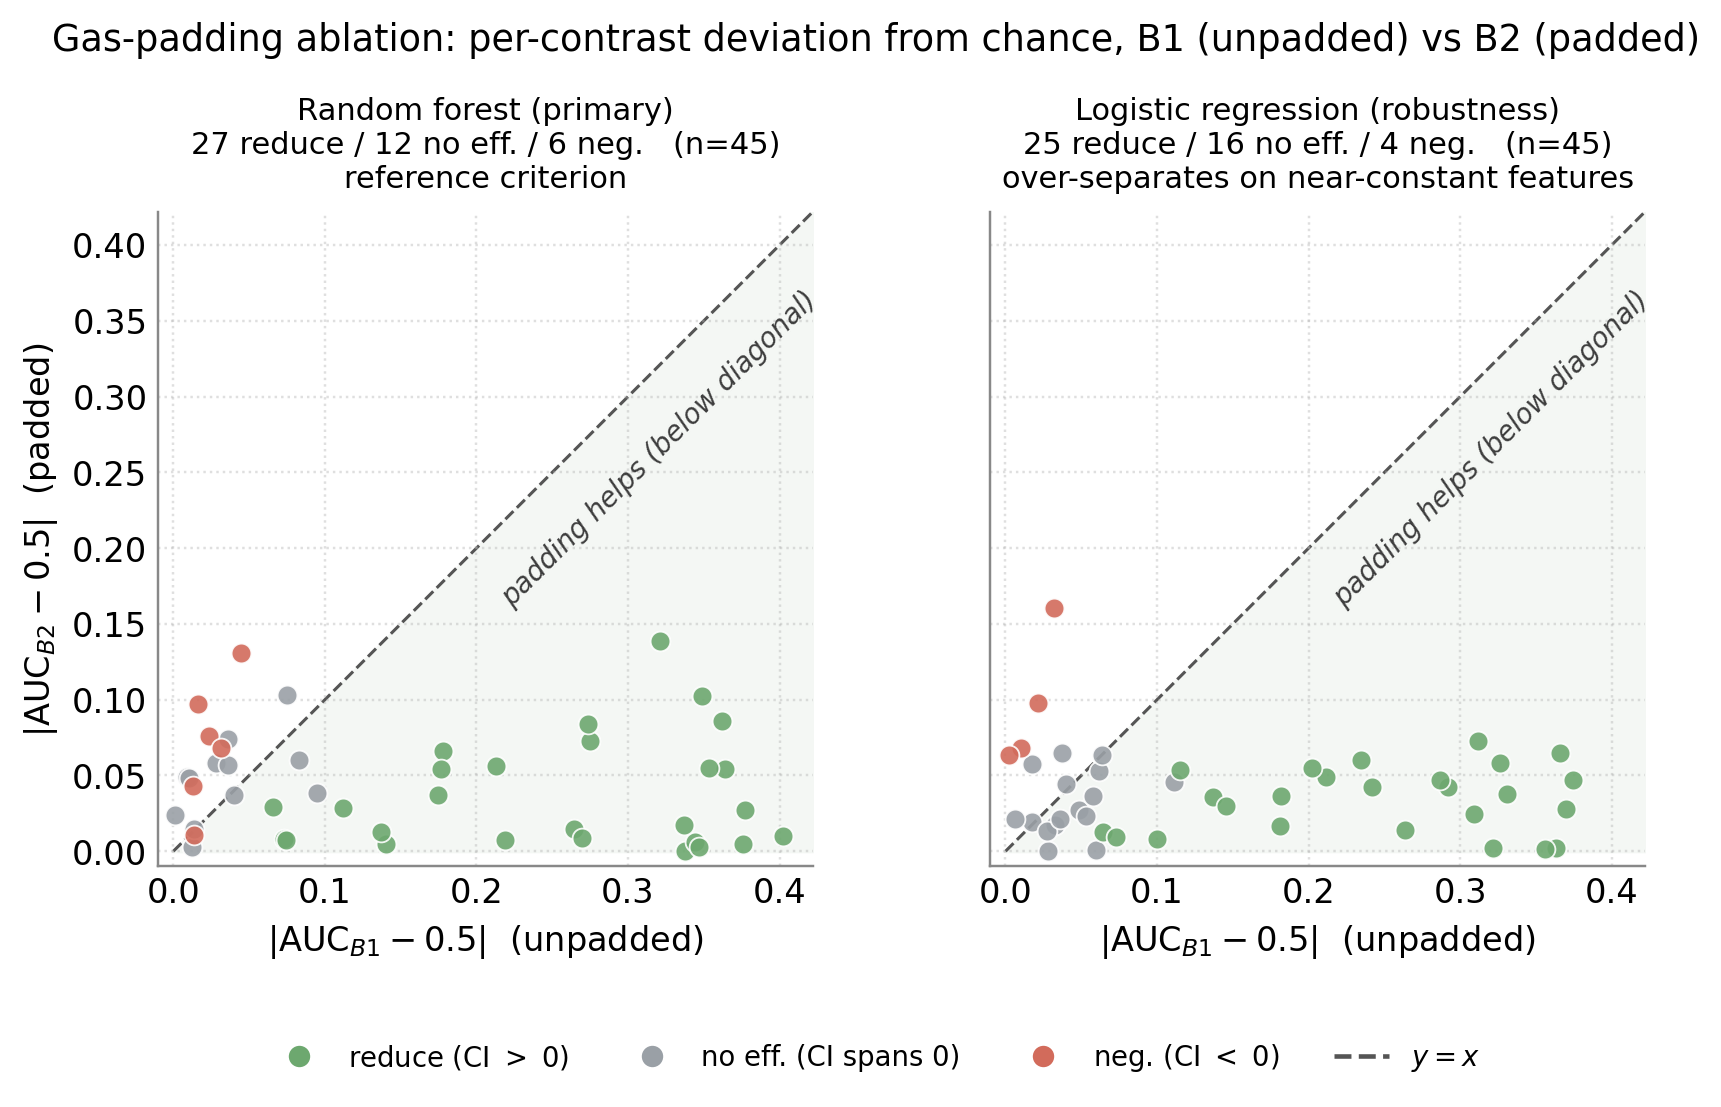
\includegraphics[width=\linewidth]{ablation_paired_scatter.png}
	\caption{Gas-padding ablation over the $45$ supervised tasks: (\textbf{a}) RF; (\textbf{b}) LR. Each point is one task, placed by the absolute deviation of its mean AUC from $0.5$ under B1 (horizontal axis) and B2 (vertical axis). Points below the dashed line $y=x$ moved closer to chance with padding. Blue, gray, and red points have $95\%$ CIs of $\Delta_{\text{leak}}$ above zero, spanning zero, and below zero, respectively.}
	\label{fig:ablation-paired}
\end{figure}

The clustering analysis provides complementary evidence.
Under B2, NMI decreases by $0.670$ for balanced PI pairs, $0.349$ for DUO terms, and $0.102$ for logical structure, with all three bootstrap confidence intervals excluding zero (Table~\ref{tab:ablation-gas-padding}).
With padding, NMI is at most $0.020$ for all three targets.

We next examine the source of the gas differences under B1.
Across the $1{,}119$ executions, unpadded access gas ranges from $723{,}288$ to $723{,}564$, excluding the first cold-start call.
Calldata analysis identifies two main sources of label-correlated variation arising from zero- and non-zero-byte pricing~\cite{akhunov2019eip2028}.
Different requester-pseudonym encodings produce an observed $192$-gas gap associated with profile-predicate use.
Sequential policy and resource identifiers introduce a further $24$-gas difference correlated with logical structure because policies were committed in groups by logical form.

Padding compensates for these calldata-pricing differences by bringing transaction gas consumption to the sampled target.
The remaining overhead varies by less than $100$ gas (Section~\ref{sec:eval-pch}), while the target varies by $\pm 105{,}000$ gas.
This provides a mechanism-level explanation for the reduced separability observed under B2.


% Single-point DEPTH=64 cost profile of the evaluated prototype configuration.
% R1CS source: protocol/releases/v3.0.0-rc2.json (constraints, wires).
% Transaction/timing source: experiments/data/polygonAmoy/executed_dataset.json
% (1977 executions of the unpadded capture of 2026-10-15, v3.0.0-rc2 artifacts; means of
% features.{commitGasUsed, accessGasUsed, proofWitnessTime, proofProveTime}; calldata and log
% sizes are constant).
\begin{table}[htbp]
	\centering
	\caption{Single-point cost profile of the evaluated prototype configuration at $L=64$.
		Gas, logs, calldata, and local prover timings are summarized over the $1{,}977$ Polygon Amoy executions.}
	\label{tab:cost-profile}
	\footnotesize
	\begin{tabular}{p{0.34\linewidth}p{0.54\linewidth}}
		\toprule
		Metric              & Value / source                                                    \\
		\midrule
		Circuit size        & $81{,}980$ constraints; $81{,}124$ wires; $L=64$        \\
		Public interface    & $4$ public inputs plus $1$ output                                 \\
		On-chain gas        & Commit $219{,}757$; access $723{,}565$ mean gas                   \\
		Event logs          & Commit: $1$ log / $180$ bytes; access: $2$ logs / $296$ bytes     \\
		Calldata length     & Commit $164$ bytes; access $580$ bytes (constant across policies) \\
		Local witness time  & $1{,}140.0$ ms mean                                               \\
		Local prove time    & $3{,}990.3$ ms mean                                               \\
		\bottomrule
	\end{tabular}
\end{table}

% Source of record: experiments/results/cost/scalability_sweep.json
% Apple M1 (8 cores), rapidsnark, 30 verified proofs per row. Timing cells are
% median [IQR] (p95), in milliseconds. Artifact sizes use decimal MB, as in the
% generated Markdown report.
\begin{table}[htbp]
  \centering
  \caption{Offline circuit-capacity sweeps (30 verified proofs per row). Timing
    cells report median [IQR] (p95) in ms; every variant keeps $N=13$, $M=11$,
    $K=5$ and five public signals.}
  \label{tab:cost-scaling}
  \scriptsize
  \setlength{\tabcolsep}{2.4pt}
  \resizebox{\textwidth}{!}{%
  \begin{tabular}{llrrrrrrr}
    \toprule
    Sweep & Capacity & Constraints & Wires & WASM (MB) & zkey (MB) & Witness & Prove & Verify \\
    \midrule
    \multicolumn{9}{l}{\emph{Program capacity: Merkle levels fixed at 8; mixed policy}}\\
    $\DEPTH$ & $32$  & $64{,}945$  & $64{,}441$  & $8.6$ & $38.7$ & $285[16](343)$ & $411[46](562)$ & $11[3](16)$ \\
    $\DEPTH$ & $64$  & $81{,}740$  & $80{,}884$  & $8.7$ & $52.2$ & $350[31](414)$ & $521[44](761)$ & $11[2](22)$ \\
    $\DEPTH$ & $128$ & $134{,}009$ & $132{,}449$ & $10.1$ & $87.5$ & $535[25](682)$ & $734[51](984)$ & $11[2](15)$ \\
    \addlinespace
    \multicolumn{9}{l}{\emph{Ontology capacity: $\DEPTH=64$; five-slot ontology-heavy policy}}\\
    Merkle levels & $4$  & $73{,}876$ & $73{,}052$ & $8.6$ & $48.3$ & $352[29](415)$ & $512[53](605)$ & $11[2](17)$ \\
    Merkle levels & $8$  & $81{,}740$ & $80{,}884$ & $8.7$ & $52.2$ & $347[3](354)$  & $499[13](539)$ & $11[1](16)$ \\
    Merkle levels & $12$ & $89{,}604$ & $88{,}716$ & $8.7$ & $56.0$ & $358[7](395)$  & $552[38](632)$ & $10[1](15)$ \\
    Merkle levels & $16$ & $97{,}468$ & $96{,}548$ & $8.7$ & $59.9$ & $370[4](456)$  & $571[38](713)$ & $10[1](13)$ \\
    \bottomrule
  \end{tabular}}
\end{table}

% Source of record: experiments/results/cost/scalability_sweep.json
% Apple M1 (8 cores), rapidsnark, RC1 circuit (DEPTH=64, MERKLE_LEVELS=8).
% (a) 30 verified proofs per policy and (b) 100 verified requests per concurrency
% level, each after five warm-ups; timing cells are median (p95) in ms, and the
% IQRs are in the JSON. (c) is computed by scripts/render_scalability_report.js:
% instances = ceil(1.5 * average rate / 0.936), the best throughput in (b).
\begin{table}[htbp]
  \centering
  \caption{Policy-content and workload scalability of the evaluated circuit ($\DEPTH=64$,
    eight Merkle levels) on one Apple M1 host using rapidsnark.}
  \label{tab:workload-scaling}
  \footnotesize
  \begin{tabular*}{\linewidth}{@{\extracolsep{\fill}}lrrrrrr@{}}
    \multicolumn{7}{@{}l}{\emph{(a) Policy content: $30$ verified proofs per policy}} \\
    \toprule
    & & & \multicolumn{4}{c}{Time (ms): median (p95)} \\
    \cmidrule{4-7}
    Policy & Tokens & Slots & Witness & Prove & Verify & End-to-end \\
    \midrule
    Simple         & $3$  & $1$  & $354$ ($418$) & $545$ ($746$) & $12$ ($14$) & $925$ ($1170$) \\
    Ontology-heavy & $19$ & $5$  & $349$ ($391$) & $506$ ($550$) & $10$ ($12$) & $880$ ($939$) \\
    Profile-heavy  & $31$ & $1$  & $337$ ($349$) & $492$ ($522$) & $10$ ($11$) & $1479$ ($1516$) \\
    Max-mixed      & $61$ & $11$ & $335$ ($346$) & $484$ ($537$) & $10$ ($10$) & $1468$ ($1538$) \\
    \bottomrule
  \end{tabular*}

  \vspace{0.8em}
  \begin{tabular*}{\linewidth}{@{\extracolsep{\fill}}ccc@{}}
    \multicolumn{3}{@{}l}{\emph{(b) Load: $100$ verified requests per concurrency level, rotating the four policies of (a)}} \\
    \toprule
    Concurrency $c$ & Throughput (proofs/s) & Latency (ms): median (p95) \\
    \midrule
    $1$ & $0.805$ & $1230$ ($1659$) \\
    $2$ & $0.787$ & $2492$ ($3805$) \\
    $4$ & $0.936$ & $4113$ ($5854$) \\
    \bottomrule
  \end{tabular*}

  \vspace{0.8em}
  \begin{tabular*}{\linewidth}{@{\extracolsep{\fill}}rrrrr@{}}
    \multicolumn{5}{@{}l}{\emph{(c) Scenarios: capacity $0.936$ proofs/s from (b); $1{,}056{,}674$ gas per padded access at $30$~gwei}} \\
    \toprule
    Accesses & Average & Prover & Access gas & Access cost \\
    per day & requests/s & instances$^{\dagger}$ & per day (billion) & (POL/day) \\
    \midrule
    $1{,}000$   & $0.012$ & $1$ & $1.057$   & $31.70$ \\
    $10{,}000$  & $0.116$ & $1$ & $10.567$  & $317.00$ \\
    $100{,}000$ & $1.157$ & $2$ & $105.667$ & $3170.02$ \\
    \bottomrule
  \end{tabular*}

  \vspace{0.4em}
  \begin{minipage}{\linewidth}
    \footnotesize\textit{Note:} Tokens: program length $\ell$ (at most $\DEPTH=64$); slots: external-predicate slots the policy uses (of $M=11$). End-to-end time also includes off-circuit evidence preparation. Latency is each request's processing time while up to $c$ requests run at once; queueing is excluded. All timings follow five warm-up requests. $^{\dagger}$Identical prover instances, $\lceil 1.5\,r/0.936\rceil$ for average request rate $r$ ($50\%$ capacity headroom). One policy commit costs $304{,}098$ gas ($0.009$~POL) and is not included, because no commit/access ratio is assumed.
  \end{minipage}
\end{table}



\section{Discussion}
\label{sec:discussion}

The evaluation indicates that TPS-ZKPI reduces the policy-dependent signals in normalized public-chain artifacts below our multi-seed leakage criterion.
Across all PCH, PI, and SPP tasks, supervised classifiers stay below that criterion, and unsupervised clustering shows no recoverable structure: ARI stays within $\pm 0.002$ of chance on every target, and the one elevated NMI (ICD-10) is consistent with the finite-sample inflation quantified by the null simulation of Section~\ref{sec:eval-nmi-sensitivity}.
The gas-padding ablation (Section~\ref{sec:eval-ablation}) sharpens this conclusion: the same attacks become measurably effective once gas padding is removed.
This attributes the gas-channel protection specifically to randomized gas padding.
Content hiding itself rests on the commitment-only interface and the content-independent transcript normalization, with padding additionally suppressing the residual gas-channel signal that is otherwise recoverable for some content labels.
Together with fixed-length policy representation, reusable interpretation, and commitment
binding, these mechanisms limit the extent to which public-chain observers infer hidden policy content or structural properties from authorization transactions.

These results support a scoped privacy claim.
The evaluation focuses on a metadata-only public-chain adversary that observes commitments, proofs, public parameters, calldata, events, and gas-related artifacts, but not TPS-side witness construction or off-chain policy material.
Within this scope, the residual cost is the randomized padding's gas overhead: about $38\%$ on access gas and $40\%$ on commit gas (Section~\ref{sec:eval-ablation}).

Boundary cases above the $0.55$ AUC line do occur---PCH chapters ch6 and ch7, and the PI \texttt{semantic\_equivalent} pairs---but none reproduces across seeds, and we report them. Stronger adversaries---compromised proof services, adaptive requester-side probing, or off-chain side channels---remain outside this scope and motivate the reduced-trust extensions discussed below.

The TPS trust assumption is the main architectural tradeoff.
Moving confidentiality-sensitive proof generation to the TPS keeps policy-bound proving information away from requesters and public smart contracts while preserving on-chain verifiability, but it shifts part of the confidentiality burden to the service layer; the provider-operated TPS used here concentrates that burden at the provider rather than at an independent service (Section~\ref{sec:problem}).
This tradeoff leaves on-chain verifiability intact but does affect liveness and accountability: the TPS or provider can refuse to produce a proof, and such a refusal may be indistinguishable from a legitimate denial at the on-chain interface.

Attribute origin is only partially delegated to the TPS.
For the profile-backed DUO terms, the circuit verifies the EdDSA-Poseidon signature described in Section~\ref{sec:design} and derives eight policy attributes from the seven signed claims.
A compromised TPS cannot modify the signed claims, policy commitment, requester pseudonym, resource, validity interval, or credential identifier without invalidating the signature.
The implemented relation rejects a non-committed issuer, an invalid signature under the committed key, an expired or premature credential, and substitutions of any signed field.
Other evidence has a narrower meaning: ontology proofs establish that a supplied code belongs to a provider-committed set, and requester allowlists establish that a holder pseudonym belongs to a provider-committed list; they do not authenticate every underlying real-world fact.
Moreover, because the TPS receives the holder secret and credential witness in the current workflow, holder binding does not protect against a malicious TPS reusing otherwise valid evidence within its signed scope.

The remaining trust anchor is therefore issuer governance.
The prototype binds the proof to a policy-selected issuer-key commitment, but it has no independent registry establishing that this key belongs to an accredited healthcare authority, and it does not check credential revocation.
The evaluation uses a deterministic test-only issuer key to exercise the complete signature path; it is not evidence of institutional issuance or production key management.

A concrete deployment can close this gap without changing the Boolean interpreter.
First, a governed issuer registry would publish schema-qualified issuer keys and their validity epochs; registration would validate a canonical, subgroup-safe public key and require proof of possession.
Second, an issuer would sign a domain-separated credential containing a holder-key commitment, claim vector, authorization scope, validity interval, and unique credential identifier.
Third, the circuit would verify both the credential signature and a Merkle proof that the issuer key is active in the registry, while continuing to derive policy attributes from the signed claims.
The holder would retain its secret key and authorize each request by signing the context digest and request epoch; verifying this second signature inside the circuit would prevent a TPS that observes one credential presentation from generating proofs for fresh sessions.
Finally, an epoch-specific sparse-Merkle or accumulator root would support a private non-revocation witness for the credential identifier.
The registry and revocation roots can occupy fixed-format public or committed parameter slots, preserving the policy-independent verification interface.
If an existing healthcare credential uses a non-circuit-friendly signature such as Ed25519 or ECDSA, integration requires either verifying that signature in-circuit at higher constraint cost or having the issuer additionally issue a SNARK-friendly credential; re-signing by the TPS would not preserve issuer-origin assurance.

As described in Section~\ref{sec:design}, the policy commitment covers both the padded encoding $P_{\mathrm{enc}}$ and its active length $\ell$.
Because $\ell$ also determines how many tokens the interpreter evaluates, an authorizing proof for $h$ cannot be based on a shorter valid prefix.
This integrity guarantee is separate from our privacy evaluation, which measures whether public-chain artifacts reveal information about the hidden policy.

The authorization context is likewise part of the proved relation.
The circuit constrains the public digest $d_{\chi}$ to the requester identifier, resource, and nonce used in the witness, and the ACM recomputes the same digest from the transaction parameters.
Consequently, changing any of these values invalidates the request.


The guarantee is scoped to the bound tuple within one ACM deployment.
The digest does not include the transaction submitter or a chain/contract domain, so exact-context front-running and cross-deployment reuse require separate deployment-level controls.
Moreover, $\mathit{id}_{\mathrm{req}}$ is a pseudonymous authorization identifier and is not, by itself, proof of a real-world identity or of the origin of every private attribute.

Three directions follow.
First, adding an explicit chain/contract domain and an authenticated submission channel would extend context binding beyond a single deployment and reduce front-running risk.
Second, accountable proof obligations---for example, on-chain commitments to serve requests together with timeout-with-evidence mechanisms---would make proof refusals attributable.
Third, the reduced-trust TPS instantiations of Section~\ref{sec:problem} (collaborative-SNARK or TEE-backed proving) would relax the trust concentration itself, including the attribute-origin limitation; realizing and evaluating them is left to future work.

\section{Conclusion}
\label{sec:conclusion}

This paper studied policy-private consent enforcement in blockchain-based
healthcare data sharing under public-chain observability and an explicit TPS trust
assumption. We proposed TPS-ZKPI,
a Trusted Proof Service-assisted zero-knowledge approach that binds hidden
provider-defined policies to on-chain commitments, evaluates Boolean-based consent
policies through a reusable policy interpreter, and normalizes public
verification artifacts to reduce metadata-level leakage. Across supervised and
unsupervised attacks on PCH, PI, and SPP, no modeled adversary recovered hidden
policy information reproducibly above chance under our multi-seed leakage
criterion, and a paired gas-padding ablation attributed the gas-channel
protection specifically to randomized gas padding---at a gas overhead of about
$38\%$ on access and $40\%$ on commit.

These results hold for a metadata-only public-chain adversary, and the privacy
claim is empirical rather than information-theoretic. Two soundness gaps in the
current instantiation remain open: the committed policy does not bind the program
length, and the proof statement is not bound to the session context
(Section~\ref{sec:discussion}). Closing both, together with extending the analysis
to stronger adaptive adversaries, off-chain leakage, richer policy languages,
reduced-trust proof generation, and privacy-preserving resource discovery, is left
to future work.


%=================================================================
% Back matter. TODO(author): every statement below is a placeholder.
\vspace{6pt}

% TODO(author): assign CRediT roles per author. See
% https://img.mdpi.org/data/contributor-role-instruction.pdf
\authorcontributions{TODO.}

% TODO(author): name the funder and grant number, or use the exact sentence
% ``This research received no external funding''.
\funding{TODO.}

% TODO(author): confirm. This is a computational study over synthetic consent
% policies with no human or animal subjects, so ``Not applicable'' is expected.
\institutionalreview{Not applicable.}

% TODO(author): confirm, same reasoning as above.
\informedconsent{Not applicable.}

% The review build (revision round 2/tools/anonymize.py) withholds this link.
\dataavailability{The source code of TPS-ZKPI (zero-knowledge circuit, smart contracts, and Trusted Proof Service), the evaluation scripts, the synthetic consent-policy corpus, and the executed dataset supporting the reported results are openly available in Zenodo at \url{https://doi.org/10.5281/zenodo.21335228}. The Polygon Amoy transactions in the executed dataset can also be checked on the public testnet.}

% TODO(author): confirm, or declare the competing interest.
\conflictsofinterest{The authors declare no conflicts of interest.}

%=================================================================
% Abbreviations. MDPI renders this via \abbreviations in the back matter.
\abbreviations{Abbreviations}{
The following abbreviations are used in this manuscript:

\begin{longtable}{@{}ll@{}}
ABAC & Attribute-Based Access Control \\
ABE & Attribute-Based Encryption \\
ACM & Access-Control Manager \\
ARI & Adjusted Rand Index \\
AUC & Area Under the Receiver Operating Characteristic Curve \\
CI & Confidence Interval \\
CP-ABE & Ciphertext-Policy Attribute-Based Encryption \\
DUO & Data Use Ontology \\
ECDSA & Elliptic Curve Digital Signature Algorithm \\
EdDSA & Edwards-curve Digital Signature Algorithm \\
EIP & Ethereum Improvement Proposal \\
EVM & Ethereum Virtual Machine \\
GA4GH & Global Alliance for Genomics and Health \\
HANCESTRO & Human Ancestry Ontology \\
HE & Homomorphic Encryption \\
ICD-10 & International Classification of Diseases, 10th Revision \\
IoMT & Internet of Medical Things \\
LR & Logistic Regression \\
MONDO & Mondo Disease Ontology \\
MPC & Multi-Party Computation \\
NMI & Normalized Mutual Information \\
OBI & Ontology for Biomedical Investigations \\
PCH & Policy Content Hiding \\
PI & Policy Indistinguishability \\
PRE & Proxy Re-Encryption \\
RF & Random Forest \\
RPN & Reverse Polish Notation \\
SAML & Security Assertion Markup Language \\
SNARK & Succinct Non-interactive Argument of Knowledge \\
SNOMED CT & SNOMED Clinical Terms \\
SPP & Structure and Parameter Privacy \\
SSI & Self-Sovereign Identity \\
TEE & Trusted Execution Environment \\
TPS & Trusted Proof Service \\
TPS-ZKPI & Trusted Proof Service-assisted Zero-Knowledge Policy Interpreter \\
WASM & WebAssembly \\
XACML & eXtensible Access Control Markup Language \\
zkVM & Zero-Knowledge Virtual Machine \\
\end{longtable}
}

%=================================================================
\appendixtitles{yes}
\appendixstart
\appendix
% Sample-size sensitivity of NMI under a null where all classes are i.i.d.
% Source of record: experiments/analysis/clustering/nmi_null_simulation.py (seed 20260923)
%   -> experiments/results/clustering/null/nmi_null_simulation.{json,md}; T=1000 per row.
% Supports the clustering cross-check (Section~\ref{sec:eval-clustering}): explains why
% small-sample NMI can be elevated even with no class-distinguishing signal.
\section{Sample-Size Sensitivity of NMI}
\label{app:nmi-sensitivity}

The clustering cross-check reads ARI directly but debiases the NMI of the balanced PI pairs (Section~\ref{sec:eval-method}).
To examine that choice, we quantify how \emph{finite-sample effects} alone can inflate NMI
even when there is \emph{no} discriminative signal, using an idealized null in which all
classes are statistically indistinguishable.

We sample every class from the \emph{same} distribution, $z_{i}\sim\mathcal{N}(0,I_{d})$ for all classes, where $I_d$ is the $d$-dimensional identity covariance and $d=2$ matches the two gas features the clustering uses.
Since no class carries class-specific information, a clustering algorithm should not recover class membership,
and both NMI and ARI should concentrate around $0$ as the sample size grows.

For each configuration we run $T=1000$ independent trials.
In each trial we
(i)~generate $G$ classes with $n$ i.i.d.\ samples per class from $\mathcal{N}(0,I_d)$, for $n_{\mathrm{tot}}=Gn$ samples in total, assigning each sample a class label by construction order (these labels are independent of the sample values, since all classes share one distribution),
(ii)~standardize the pooled data and apply K-Means with $K=G$ and ten initializations, as in the evaluation, and
(iii)~score the predicted assignments against these assigned class labels with NMI and ARI.
We vary $n$ while holding $G$ fixed, and report the trial means $\overline{\mathrm{NMI}}$ and $\overline{\mathrm{ARI}}$.
We consider a \textbf{PI-like} binary structure ($G=2$, $n\in\{3,10,50,100\}$), a five-class structure ($G=5$, $n\in\{3,10,100\}$), and a ten-class structure ($G=10$, $n\in\{3,10,77\}$) together with the observed ICD-10 chapter sizes ($49$--$135$ executions per chapter, $n_{\mathrm{tot}}=770$).

Table~\ref{tab:nmi-sample-size-sensitivity} shows that, although all classes are indistinguishable by construction, \textbf{NMI is noticeably positive at very small $n$ but collapses toward zero as $n$ grows}, whereas \textbf{ARI stays near zero throughout}.
For the binary structure, $\overline{\mathrm{NMI}}$ falls from $0.2074$ at $n=3$ ($n_{\mathrm{tot}}=6$) to $0.0420$ at $n=10$, and to $0.0072$/$0.0034$ at $n=50$/$100$.
The same trend holds with more classes, at a higher level for every $n$: with five classes $\overline{\mathrm{NMI}}$ goes from $0.4152$ ($n=3$) to $0.0102$ ($n=100$), and with ten classes from $0.5346$ ($n=3$) to $0.0239$ ($n=77$).
For the observed ICD-10 chapter sizes, a separate null run that averages each trial over $20$ K-Means seeds, as the evaluation does, gives a null NMI with mean $0.0246$ and $95$th percentile $0.0302$; the observed ICD-10 NMI of $0.0281$ is reached in $145$ of $1000$ null trials ($p=0.15$).

\begin{table}[htbp]
	\centering
	\caption{Sample-size sensitivity of NMI and ARI under the null hypothesis where all
		classes are i.i.d.\ sampled from $\mathcal{N}(0,I_d)$.}
	\label{tab:nmi-sample-size-sensitivity}
	\begin{tabular*}{0.54\linewidth}{@{\extracolsep{\fill}}rrrr@{}}
		\toprule
		$n$ (per class) & $n_{\mathrm{tot}}$ & $\overline{\mathrm{NMI}}$ & $\overline{\mathrm{ARI}}$ \\
		\midrule
		\multicolumn{4}{@{}l}{\textit{Two classes (as in a PI pair)}} \\
		$3$       & $6$   & $0.2074$ & $0.0127$  \\
		$10$      & $20$  & $0.0420$ & $0.0008$  \\
		$50$      & $100$ & $0.0072$ & $-0.0003$ \\
		$100$     & $200$ & $0.0034$ & $-0.0004$ \\
		\addlinespace
		\multicolumn{4}{@{}l}{\textit{Five classes}} \\
		$3$       & $15$  & $0.4152$ & $-0.0034$ \\
		$10$      & $50$  & $0.1226$ & $0.0003$  \\
		$100$     & $500$ & $0.0102$ & $-0.0000$ \\
		\addlinespace
		\multicolumn{4}{@{}l}{\textit{Ten classes (as the DUO and ICD-10 targets)}} \\
		$3$       & $30$  & $0.5346$ & $-0.0009$ \\
		$10$      & $100$ & $0.2087$ & $0.0003$  \\
		$77$      & $770$ & $0.0239$ & $-0.0001$ \\
		\addlinespace
		\multicolumn{4}{@{}l}{\textit{Ten classes, observed ICD-10 chapter sizes}} \\
		$49$--$135$ & $770$ & $0.0244$ & $-0.0001$ \\
		\bottomrule
	\end{tabular*}

	\begin{tablenote}
		$T=1000$ trials per row, one K-Means fit with ten initializations per trial; $n_{\mathrm{tot}}$ is the total sample size.
		For the observed ICD-10 chapter sizes, the text also reports a separate run that averages each trial over $20$ K-Means seeds, as the evaluation does.
	\end{tablenote}
\end{table}


% Output any appendix float still pending here, so that it cannot drift into the
% reference list; this starts a new page only if a float would otherwise move past.
\FloatBarrier

%=================================================================
\begin{adjustwidth}{-\extralength}{0cm}

\reftitle{References}
\bibliography{reference}

\PublishersNote{}
\end{adjustwidth}
\end{document}
